\documentclass[12pt,a4paper]{article}
\usepackage[utf8]{inputenc}
\usepackage[T1]{fontenc}
\usepackage{amsmath}
\usepackage{amsfonts}
\usepackage{amssymb}
\usepackage{graphicx}
\usepackage{hyperref}
\usepackage{setspace}
\usepackage{titlesec}
\usepackage{booktabs}
\usepackage{array}
\usepackage{longtable}
\usepackage{float}
\usepackage{tikz}
\usepackage{pgfplots}
\pgfplotsset{compat=1.17}
\usepackage{tcolorbox}

% Use the page.sty styling
\usepackage{page}

% Use biblatex with ref.bib
\usepackage[style=numeric]{biblatex}
\addbibresource{ref.bib}

\onehalfspacing

\hypersetup{
    colorlinks=true,
    linkcolor=blue,
    filecolor=magenta,      
    urlcolor=cyan,
    citecolor=blue
}

\begin{document}

\begin{titlepage}
\begin{center}
\vspace{3cm}

\includegraphics[scale=0.5]{assets/JADS_logo.png}\\
%\LARGE
%Eindhoven University of Technology \\
\large
% Department of Mathematics and Computer Science  \\
% Architecture of Information Systems Research Group

\vspace*{1cm}

\setlength{\TPHorizModule}{1mm}
\setlength{\TPVertModule}{\TPHorizModule}
% Set the Paragraph Indent to zero, so the first line is not Indented
% Back-up the current value so it can be put back at the end of the title page
\newlength{\backupparindent}
\setlength{\backupparindent}{\parindent}
\setlength{\parindent}{0mm}		

% Begins a textbox at 72 mm from the left of the edge of the paper and 89 mm from the top
% The width of the textbox is 95 mm (167 - 72 mm)
% The height of the box cannot be defined, so it is your task to keep the text not too long
	
{ \huge \sc Engineering Doctorate in }\\[0.55cm]
{ \Huge \sc Data Science
}\\[0.45cm]
\vspace{3cm}

\LARGE
\textbf{\doctitle \\}
\vfill
\begin{textblock}{95}(58,180)
    \vspace*{2mm}
    \large
    \vspace*{30mm}
    \textbf{\ Prepared by:}
    \Large\\
    \begin{tabular}{cl}
        Kenneth Mwandingi
    \end{tabular}\\
    \vspace*{8mm}
    \large
    \textbf{\ Prepared for:}\\ TU/e and JADS

     
    \normalsize
    \vfill
\vspace*{10mm}
\large
% \DTMdate{2024-06-01}
\today
    
\end{textblock}

% \large
% Supervisors:\\
% \begin{tabular}{rl}
%     \firstCommitteeMember\\
%     \secondCommitteeMember\\
%     \thirdCommitteeMember\\
% \end{tabular}

\vfill
% \version
\vfill
%\docdate \\
%\large
%\bigskip
 %\textbf{\text{`}s-Hertogenbosch}\\
%\datemonthyear

% Put the Paragraph Indent back to its original value
\setlength{\parindent}{\backupparindent}
\end{center}
\end{titlepage} 



\clearemptydoublepage
\noindent{\Large\bfseries EngD report INFORMATION}\\

\vspace{0.1cm}
\noindent
Kenneth Mwandingi

\vspace{0.4cm}
\noindent
Eindhoven University of Technology \\
Jheronimus Academy of Data Science \the\year{} .  \\    
Report of the Engineering Doctorate (EngD) program: \\
Data Science EngD report number: \the\year{}/00? \\
Keywords: energy management system, dynamic pricing, machine learning, mixed-integer linear programming, optimization, building-level optimization, agent-based design, probabilistic modeling

\vspace{0.4cm}

\noindent{\bfseries Composition of the Thesis Evaluation Committee}\\
\noindent
Company supervisors:  \\
% List your company supervisors here

\noindent
Scientific supervisor:  \\
% List your scientific supervisor here

\noindent
Independent members:  \\
% List committee members here

\noindent
Chair of the committee:  \\
% List committee chair here

\vspace{0.4cm}
\noindent
The design described in this thesis has been carried out in accordance with the TU/e code of Scientific Conduct

\vspace{0.4cm}
\noindent
\textcopyright\ 2025, Eindhoven University of Technology

\vspace{0.4cm}
\noindent
Niets van deze uitgave mag worden vermenigvuldigd en/of openbaar 
gemaakt worden door middel van druk, fotokopie, microfilm of op welke
andere wijze dan ook zonder voorafgaande schriftelijke toestemming 
van de auteur.

\vspace{0.4cm}
\noindent
No part of this publication may be reproduced or transmitted in any 
form or by any means, electronic or mechanical, including photocopy, 
recording, or any information storage and retrieval system, without 
permission from the copyright owner.

\vspace{0.4cm}
\noindent
*) ISBN information only requested for the report of the final project.


\maketitle

% Abstract
\begin{abstract}
\noindent 
\textbf{Abstract –} This report presents the development of an agent-based, probabilistic Energy Management System (EMS) designed to optimize building-level energy usage under dynamic electricity pricing. The EMS integrates data-driven learning and Mixed-Integer Linear Programming (MILP) optimization in a modular architecture. The key novelty is the use of probabilistic models of appliance usage to inform scheduling decisions. This approach allows the system to anticipate occupant behavior and handle uncertainty better than deterministic approaches. 

The multi-agent design includes specialized agents for photovoltaic (PV) generation, battery storage, electric vehicles (EVs), flexible appliances, and a global optimizer. This architecture enables scalability and flexibility across different building configurations. Each evening, a day-ahead optimal schedule is computed for all controllable devices using next-day price forecasts. Intraday updates are performed as new data (actual usage, solar irradiance, etc.) arrives. 

Simulation results on representative scenarios demonstrate significant benefits. The EMS achieves electricity cost reductions on the order of 10–36\% for typical households without storage, with even greater savings when battery storage is present. It substantially increases PV self-consumption (from about 40\% to 85–95\%) by intelligently timing loads. The system reduces peak grid demand by 20–30\% on average, contributing to a flatter load profile and improved grid stability. 

These gains are attained while respecting user-defined comfort constraints. Over 85–90\% of appliance operations remain within preferred time windows. Computational run-times are suitable for real-world use (on the order of seconds for day-ahead scheduling). The results highlight the potential of AI-driven, probabilistic energy management to lower costs for end-users, enhance renewable energy utilization, and provide demand flexibility for the grid. 

The agent-based approach proved crucial for modularity and resilience. The system can easily incorporate new device types or adapt to different markets (e.g., integrating real-time pricing or future grid services). In summary, the proposed EMS framework shows a viable path toward smarter, cost-effective, and user-centric energy management in buildings under dynamic pricing.
\end{abstract}

\newpage
\tableofcontents
\newpage

\section{Executive Summary}

\noindent 
This report describes the design and implementation of an AI-enabled Energy Management System (EMS) for optimizing building energy consumption under dynamic electricity pricing. The system is developed with a dual context in mind: it is prototyped and validated in the Dutch energy market – characterized by real-time and day-ahead electricity tariffs, widespread smart metering, and demand-response programs. At the same time, it is designed for future deployment in Curaçao, a Caribbean island currently using monthly flat tariffs and in the early stages of grid modernization. This dual approach ensures the solution is immediately relevant in advanced markets and future-proof for emerging smart grid environments. 

The EMS framework comprises two main components:

\textit{Part 1} is a modular system architecture that integrates data ingestion, secure communications, and user-centric interfaces. This addresses system-level challenges of aggregating data from distributed energy resources (DERs) such as flexible appliance loads, photovoltaic generation, and battery storage while maintaining robust cybersecurity and privacy. 

\textit{Part 2} is an intelligent optimization engine employing a multi-phase, multi-agent control strategy. The EMS uses a two-stage decision process that combines day-ahead scheduling with continuous intraday learning. 

Each evening when next-day electricity prices are published, the system computes an optimal 24-hour operating schedule for all controllable devices and storage. This leverages the latest forecasts (for weather and solar PV) and learned usage patterns. Throughout the following day, as real-time consumption and generation data arrive, the EMS updates its probabilistic models of device usage and adjusts control actions in a rolling manner. This adaptive cycle balances cost efficiency, user comfort, and grid reliability better than static or purely rule-based approaches.

Strategically, the EMS is part of a broader smart energy initiative bridging academic research and real-world utility needs. While initial development leverages the data-rich, dynamic pricing environment of the Netherlands, the system is explicitly designed to evolve and address local challenges in markets like Curaçao. 

Anticipated adaptations include: 
\begin{itemize}
    \item Enabling a gradual transition from flat monthly rates to granular time-of-use or real-time pricing as smart meters are deployed.
    \item Incorporating energy budgeting tools to help mitigate energy poverty for low-income households.
    \item Providing enhanced grid-balancing features to integrate higher shares of intermittent renewables (solar/wind) into the local grid.
\end{itemize} 

These goals align with policy objectives for sustainable and affordable energy (for example, Curaçao's national target of 40\% reduction in energy use by 2030). 

Preliminary simulations and pilot tests demonstrate substantial benefits of the EMS. It consistently reduces energy costs by shifting flexible loads to cheaper tariff periods, yielding electricity bill savings on the order of 12–38\% for households and commercial buildings under dynamic pricing. 

When on-site solar PV and battery storage are present, the EMS dramatically increases PV self-consumption. For example, in one test scenario the portion of solar generation utilized on-site rose from ~42\% to ~87\% through intelligent load timing. It also cuts peak grid imports (peak demand) considerably, improving grid stability.

The system maintains high user comfort/satisfaction, with $>85\%$ of appliance operations kept within user-preferred time windows. The optimization engine operates efficiently, solving the daily MILP scheduling problem in roughly 5–10 seconds per building on average. It robustly handles uncertainties in user behavior and solar output via continuous learning and adjustment. 

These results underscore the EMS's potential not only to lower costs and carbon footprint for end-users, but also to assist utilities in peak shaving and renewable integration at scale. 

In summary, the developed EMS combines advanced machine learning (to predict and adapt to human energy usage patterns) with mixed-integer linear programming (to optimally schedule devices and storage) in a novel, integrated framework. It delivers tangible value for building operators (cost savings and resilience to price spikes), for utilities (demand flexibility and new tariff opportunities), and for society (reduced emissions and progress toward energy sustainability). The system's agent-based modular design ensures scalability from single homes to multi-building complexes and adaptability across different markets and regulatory environments.

The remainder of this report is organized as follows: Section 2 provides a management introduction with background context and strategic value; Section 3 reviews the state-of-the-art in home/building energy management; Section 4 chronicles the iterative design evolution from initial concept to final probabilistic multi-agent solution; Section 5 details the technical architecture and mathematical formulation; Section 6 presents the business case and applications; Section 7 discusses evaluation results and performance metrics; and Section 8 concludes with a summary and future work directions. Together, these sections illustrate how an intelligent EMS can serve as a strategic enabler for smart grids and the sustainable energy transition in both developed and developing regions.

\clearpage

\section{Management Introduction}
Modern energy systems are undergoing rapid transformation driven by increased penetration of renewable generation, dynamic electricity pricing, and the proliferation of smart devices in homes and buildings. In advanced markets like the Netherlands, electricity prices can fluctuate on an hourly basis according to supply and demand, creating opportunities for consumers to reduce costs if they can respond to price signals (e.g. by shifting consumption to cheaper periods) \cite{Mahmoudi2020, AlSorour2022}. However, most buildings today lack automation in energy management; appliances and HVAC systems are usually operated for convenience or comfort with little regard to price variations. Consequently, building occupants often miss out on potential savings, and peak demand times remain high, straining the grid \cite{Koltsaklis2019, Chen2024}. Meanwhile, the rise of intermittent renewables like solar PV and wind is introducing new challenges: these sources do not always produce energy when consumption is highest, leading to periods of surplus generation and periods of deficit that can threaten grid stability if not managed \cite{Yoshida2018, TostadoVeliz2023}. These trends, coupled with globally rising energy costs (driven by fuel price volatility, geopolitical factors, and carbon policies), put financial pressure on consumers and demand new solutions for efficient energy usage \cite{Rehman2025, Chen2024}.

Energy Management Systems (EMS) for buildings have emerged as a promising solution to address the above challenges by intelligently coordinating when and how various devices consume or store electricity \cite{AlSorour2022, Mahmoudi2020}. A Building-level EMS (often also termed HEMS – Home Energy Management System – in residential contexts) can automatically schedule appliances, heating/cooling systems, and storage devices (like batteries or EV chargers) in response to price signals and renewable availability. For example, an EMS might delay an electric water heater or EV charging from peak-price evening hours to low-price overnight hours, as long as user-defined comfort constraints are met (hot water is ready by morning, car battery is full by departure time, etc.) \cite{Yoshida2018, TostadoVeliz2023}. By doing so across all major flexible loads in a building, the EMS reduces the total energy bill and flattens the demand curve, benefiting both the end-user and the grid.

\subsection*{Background and Problem Statement}
In a traditional scenario without an EMS, building energy usage is often \textit{non-optimal} under dynamic pricing: devices are used whenever convenient, and on-site generation (if present) may be wasted or sold at low feed-in tariffs rather than directly utilized. This leads to several inefficiencies:
\begin{itemize}
    \item \textbf{Unnecessary Cost Expenditure:} Appliances may run during expensive peak periods when they could be shifted to cheaper times, resulting in higher electricity bills.
    \item \textbf{Low Renewable Utilization:} Without coordination, a building with solar panels might export surplus solar energy at low rates or even curtail generation, while later drawing power from the grid at high cost. The lack of alignment between solar production and load leads to low self-consumption of PV energy.
    \item \textbf{High Peak Demand:} If many devices run concurrently (especially during peak hours), the building’s peak power draw is high, contributing to grid strain and potentially incurring peak demand charges or higher tariffs. A high peak-to-average load ratio (PAR) is inefficient for the grid.
    \item \textbf{User Inconvenience vs. Savings:} If users manually try to respond to prices, it requires effort and may conflict with comfort (e.g. waiting until midnight to run the dishwasher). There is a need for automation that optimizes without sacrificing user preferences.
\end{itemize}

The problem addressed by this project is how to intelligently manage and schedule building energy resources to minimize costs and maximize efficiency under time-varying prices, while respecting user comfort and operational constraints. Key objectives include:
\begin{itemize}
    \item \textbf{Electricity Cost Reduction:} Shift or modulate energy usage to exploit lower-priced time periods (and avoid high-price periods), thereby reducing the total cost of energy for the building \cite{Mahmoudi2020, AlSorour2022}. We target double-digit percentage savings (initial simulations indicate 10–20\% bill reductions are achievable for typical homes).
    \item \textbf{Demand Peak Reduction:} Flatten the building’s load profile by avoiding unnecessary simultaneity of flexible loads, thus reducing the peak demand. Lower peaks benefit the grid by reducing strain and the need for expensive peaking power plants \cite{Koltsaklis2019, Chen2024}. In our scenario analysis, the EMS can cut household peak grid import by ~20–30\% on average \cite{Koltsaklis2019}, which if scaled across many buildings contributes to a more stable grid (see Results).
    \item \textbf{PV Self-Consumption Increase:} For buildings with rooftop solar PV, schedule controllable loads (and battery charging) to absorb excess solar generation on-site. This increases the percentage of PV energy directly used in the building, reducing reliance on grid power and improving return on investment for solar. The EMS in testing raised PV self-consumption from roughly 42\% to 87\% in one case, and some battery-equipped homes achieved near 95–100\% PV utilization \cite{Yoshida2018, TostadoVeliz2023}.
    \item \textbf{User Comfort and Preference Compliance:} Ensure that automation does not unduly hinder occupants. The EMS must respect user-specified time windows or priorities for appliance operation (for example, “finish laundry by 9 PM” or “keep living room at 21°C between 6–10 PM”). We measure user satisfaction as the percentage of appliance operations that occur within the user's preferred schedule; our goal was to exceed 85\%, which was achieved in simulations (typically 85–90+\% of operations meet preferences).
    \item \textbf{Grid and Societal Benefits:} By coordinating demand, the EMS also provides ancillary benefits: it can facilitate demand response programs (allowing users to capitalize on or contribute to grid signals), reduce emissions by better integrating renewables, and potentially alleviate energy poverty by cutting waste. For example, demand-response enabled EMS could respond to critical peak pricing or emergency events, offering aggregated load reduction to the utility \cite{Chen2024}.
\end{itemize}

\subsection*{Goals and Strategic Value}
The strategic value of this project extends beyond a single-building cost saver:
\begin{itemize}
    \item For \textbf{consumers}, it provides an automated tool to manage energy bills proactively, offering transparency (e.g. projected costs, savings achieved) and control (ability to override or set preferences). This can increase awareness of energy usage and empower users to participate in dynamic pricing markets without hassle.
    \item For \textbf{utilities and grid operators}, widespread adoption of such EMSs can provide a more flexible demand side. It effectively transforms buildings into smart assets that can shave peaks and fill valleys in demand, which is crucial as more renewable generation comes online. It opens the door for aggregated demand response, where many EMS-equipped homes collectively reduce load during grid stress events \cite{Koltsaklis2019}. It also can delay or reduce the need for grid upgrades by smoothing local load profiles.
    \item For \textbf{policy objectives}, the project aligns with sustainability and energy transition goals. By maximizing use of renewables and cutting waste, it helps reduce carbon emissions. By potentially offering energy budgeting features, it can support social goals like alleviating the burden of high energy costs on vulnerable populations. In Curaçao's context, where current infrastructure is less advanced, the EMS is purposefully designed to be adaptable – for instance, it can initially operate in a recommendation or monitoring mode until smart appliance control is feasible, and it can incorporate gradually more dynamic tariffs as they are introduced. This "future-proofing" makes the solution relevant both in high-tech and developing grid environments \cite{Rehman2025}.
\end{itemize}

\subsection*{Key Contributions}
This project makes several novel contributions to the field of building energy management:
\begin{itemize}
    \item \textbf{Probabilistic Device Modeling:} Development of a Bayesian learning framework that continuously updates probability mass functions (PMFs) of appliance usage patterns based on observed behavior, enabling the system to adapt to changing user habits.
    \item \textbf{Adaptive MILP Formulation:} Integration of learned probabilistic models directly into the mixed-integer linear programming optimization, creating a feedback loop between user behavior learning and scheduling decisions.
    \item \textbf{Multi-Agent Architecture:} Design of a modular, agent-based system where specialized agents (PV, battery, EV, flexible devices) coordinate through a global optimizer, enabling extensibility and resilience.
    \item \textbf{Dual-Market Design:} Development of an EMS framework that functions effectively in both advanced markets with dynamic pricing and emerging markets with simpler tariff structures, ensuring broad applicability.
    \item \textbf{User-Preference Balancing:} Implementation of a novel penalty-based approach that explicitly quantifies the trade-off between cost savings and user convenience, allowing for customizable comfort-cost balancing.
    \item \textbf{Continuous Learning Mechanism:} Creation of a rolling horizon optimization with daily updates to probability models, enabling the system to improve over time without requiring manual reconfiguration.
    \item \textbf{Practical Deployment Blueprint:} Demonstration of a complete implementation pathway from concept to deployment, including hardware integration specifications, software architecture, and user interface considerations.
\end{itemize}
In summary, the introduction of an agent-based probabilistic EMS addresses a timely need in today’s energy landscape: how to utilize advanced ICT (Information and Communication Technologies), machine learning, and optimization to turn buildings into active participants in the energy ecosystem. The following sections present a review of related work, the evolution of our project approach, the architecture and methodology of our solution, and a discussion of the results obtained.

\clearpage

\section{Literature Review}
Research on Home and Building Energy Management Systems (HEMS/BEMS) has expanded substantially in the past decade, reflecting the growing importance of demand-side flexibility in modern smart grids. This section reviews key trends and findings from the literature, focusing on optimization techniques for energy scheduling, methods for handling uncertainty, and integration of probabilistic models of demand.

\subsection{Optimization-Based Energy Scheduling}
Early HEMS solutions often relied on heuristic or rule-based control strategies (for example, simple if-then rules to turn off appliances during peak hours, or user-defined schedules set via smartphone apps). While straightforward, those approaches cannot guarantee cost-optimal outcomes and often neglect the complex interactions between devices. In contrast, optimization-based methods formulate the scheduling problem mathematically, capturing device constraints and cost objectives to find an optimal or near-optimal schedule. Among these, Mixed-Integer Linear Programming (MILP) has emerged as a widely used formulation technique for HEMS due to its ability to handle binary on/off decisions and linear constraints efficiently. Many studies (e.g., Al-Sorour et al. 2022; Koltsaklis et al. 2019) have applied MILP models to schedule home appliances under time-of-use or real-time pricing, showing significant cost savings compared to non-optimized usage. MILP is favored for its guarantee of finding a global optimum for the given objective and its flexibility to include various operational constraints (device operating limits, user comfort requirements, etc.). 

For instance, Al-Sorour et al. (2022) use MILP to optimally schedule household appliances and report electricity bill reductions in the range of 15–30\% under dynamic tariffs. Similarly, Dinh et al. (2022) formulated a MILP for a home with PV panels and battery storage, achieving better cost performance than both a heuristic baseline and the home’s original (unoptimized) operation, particularly by leveraging battery storage to arbitrage energy prices. These results illustrate that MILP-based HEMS can indeed yield double-digit percentage savings in practice, which validates the core approach of our project.

At the same time, MILP comes with computational challenges if the problem is very large (many devices or fine time granularity), but recent works have shown that typical residential scheduling problems are tractable with modern solvers. Our own implementation solves a day-ahead schedule (24 hours, hourly or quarter-hourly intervals, with a handful of devices and one battery) in around seconds per building on an open-source solver, which is acceptable for daily use.

\subsection{Handling Uncertainty: Robust and Stochastic Methods}
A major challenge in energy management is uncertainty in factors like user behavior (when will an occupant actually need the appliance?), renewable generation, and sometimes even real-time prices. Researchers have explored both robust optimization and stochastic (scenario-based) optimization to address these uncertainties. Robust optimization (e.g., \cite{Mahmoudi2020}) formulates the problem such that the solution is feasible under the worst-case realization of uncertainties, providing guarantees at the expense of some conservatism. For example, \cite{TostadoVeliz2023} propose a fully robust home energy management model considering real-time prices and EV battery uncertainty, ensuring that the schedule is valid for all possible price fluctuations and EV availability scenarios. Their approach yields a schedule that hedges against price spikes and EV plug-in variability, albeit at the cost of slightly higher expected cost (due to holding extra safety margin).

Stochastic optimization approaches (e.g., \cite{Yoshida2018}) instead consider multiple scenarios or probability distributions of uncertain parameters. \cite{Yoshida2018} use a stochastic optimal scheduling for HEMS, incorporating scenarios for uncertain solar generation and appliance usage, and demonstrate that a stochastic MILP can outperform a deterministic one by anticipating likely variations. These studies indicate that accounting for uncertainty (whether via robust or stochastic methods) can improve real-world performance of an EMS, especially for handling renewable intermittency and random user behavior.

Our project draws inspiration from these works by integrating uncertainty considerations through a probabilistic modeling approach. Instead of treating appliance usage or solar output as fixed inputs or worst-case bounds, we develop a Probability Model Agent that learns probabilistic profiles (distributions) of device usage times. This allows the optimization to incorporate a “likelihood” of usage in its objective or constraints (for example, penalizing schedules that deviate from typical usage patterns). It is a form of data-driven stochastic optimization, where the probabilities are learned from data rather than assumed. This approach contributes a novel angle to HEMS research: whereas many prior works assume deterministic user behavior or require scenario enumeration, our EMS continuously learns and updates usage probabilities to inform scheduling decisions.

\subsection{User Preferences and Human-in-the-Loop Considerations}
Another stream of relevant literature deals with user preferences and acceptance of automated energy systems. A key insight is that even the best energy-saving schedule will fail if it violates comfort expectations or if users feel out of control. Recent studies emphasize incorporating user satisfaction metrics and allowing manual overrides in HEMS design. For instance, \cite{Rehman2025} in a systematic literature review note a trend towards more human-centric energy management, recommending that systems learn from user habits and provide understandable feedback. Our work contributes to this trend by explicitly integrating learned probabilistic user preferences into the optimization objective (via a penalty for scheduling outside preferred times) and by designing the system architecture to accommodate user interaction (a UI layer where users can adjust preferences or override schedules). The area of translating qualitative user comfort into quantitative constraints or costs in optimization is still developing, and our project offers a case study in doing so. We show that by assigning a suitably high weight to user convenience in the objective function, the EMS can maintain very high satisfaction (85–90\% of operations within desired time windows) at a modest cost to optimality (a small increase in total energy cost, e.g. 1–3\% relative). This aligns with findings by other authors that user-friendly operation is achievable with minimal efficiency loss.

\subsection{Multi-Agent and Decentralized Control Approaches}
The concept of using multi-agent system (MAS) architectures in energy management has been explored in literature as well, especially for distributed control or peer-to-peer energy trading scenarios. While our focus is on a single-building EMS, we adopt an agent-based modular design internally. The rationale for this design choice (as also supported by general software architecture principles and some studies on MAS for microgrids) is to enhance modularity, scalability, and maintainability \cite{Chen2024}. Each functional component (forecasting, scheduling, device control) acts as an “agent” with well-defined interfaces, which aligns with the principles found in industrial control systems. Though literature specific to single-building MAS is limited, we took inspiration from concepts in both smart grid MAS research and software engineering: for example, agents allow parallel development and testing (one can improve the PV forecasting module independently from the rest) and fault isolation (if one agent fails, it can be restarted without collapsing the whole system) \cite{Koltsaklis2019}. This approach is somewhat orthogonal to the optimization algorithms themselves, but it informs how we implemented the EMS in a flexible way. 

In summary, the literature suggests that:
\begin{itemize}
    \item MILP optimization is a proven technique for HEMS and yields significant cost and energy savings.
    \item Handling uncertainty via robust or stochastic methods can improve reliability, especially for renewables and variable loads (we address this by learning probability distributions rather than assuming fixed values) \cite{Mahmoudi2020, Yoshida2018}.
    \item User-centric design (preferences, feedback, overrides) is critical for real-world adoption; our approach integrates this insight by design \cite{Rehman2025, Chen2024}.
    \item Modular, agent-based architectures can enhance system scalability and resilience, supporting the integration of new devices or features over time \cite{Chen2024, Koltsaklis2019}.
\end{itemize}

\paragraph{Gap in the Literature} Despite these advances, our review identified several key gaps in existing research. First, most HEMS implementations treat user behavior as either deterministic or as a static probability distribution, failing to adapt to changing usage patterns over time. Second, while many systems optimize for either cost or user comfort, few provide a systematic framework for balancing these competing objectives with tunable parameters. Third, there is limited research on systems that can function effectively across different market structures (from advanced dynamic pricing to simpler time-of-use tariffs). Our EMS addresses these gaps through its adaptive probabilistic learning, preference-weighted optimization framework, and market-agnostic design principles.

This project builds upon and combines these insights, aiming to contribute a novel integrated solution. In the next section, we discuss how the project concept was ideated and evolved, including key decisions influenced by both the literature and practical considerations.

\clearpage

\section{Project Ideation and Evolution}
The development of the EMS followed an iterative process, with the project scope and approach evolving based on initial findings, stakeholder feedback, and practical constraints. This section outlines the major evolution points and design decisions that shaped the final solution across three distinct phases.

\subsection{Phase 1: Initial Concept and Scope}
At the project’s outset, the vision was broad: to create a comprehensive digital energy assistant for buildings, incorporating detailed forecasting, optimization, and even occupant interaction. Early on, we brainstormed a system that would not only optimize in response to prices (price-driven demand response) but also include predictive capabilities for the building’s baseline (inflexible) energy usage. The idea was that if one could forecast the "must-run" load (e.g. base HVAC or plug loads that are not shiftable), the EMS could better schedule the flexible part around it \cite{Mahmoudi2020, AlSorour2022}. We also considered extending the scope beyond a single building to a network of buildings (community energy management), where the EMS could facilitate energy sharing or peer-to-peer trading among neighbors.

However, as the project progressed, we had to balance ambition with feasibility. One of the first scope refinements was to \textbf{deprioritize explicit baseline demand forecasting}. Predicting a building’s non-shiftable load (e.g. exact HVAC usage) can be as complex as the core scheduling problem itself and could divert focus. Instead, we decided to treat non-controllable loads as given inputs (using historical averages or simple extrapolation) and focus our modeling efforts on the controllable devices and PV generation. This shift was partly due to time constraints and the recognition that building a top-notch general load forecaster could be a full project on its own. By assuming the inflexible part of the load profile is approximately known or constant (or that its uncertainty can be handled in aggregate by slight re-optimization each day), we kept the project manageable. In implementation, we simply use a baseline profile (from historical data) for the inflexible load and update it periodically; any errors in that baseline would be compensated by the next day’s optimization.

\subsection{Phase 2: Adoption of an Agent-Based Architecture}
Another major evolution was the decision to structure the EMS as an \textbf{agent-based modular system} instead of a monolithic application. Initially, the team considered building the EMS as one integrated program that ingests all inputs (prices, sensor data, etc.) and outputs device schedules in one block. However, drawing inspiration from industrial control systems and multi-agent systems literature, we opted for a more modular architecture early in the design. In this architecture, each functional element of the system (forecasting, optimization, device control, user interface, etc.) is encapsulated in an independent “agent” with well-defined interfaces. 

This decision was justified by several reasons:
\begin{itemize}
    \item \textbf{Modularity and Parallel Development:} Different team members (or future developers) can work on separate agents simultaneously. For example, one subgroup could focus on improving the ProbabilityModel agent (tweaking the learning algorithm for appliance usage) while another works on the GlobalOptimizer MILP formulation, with a clear contract of data exchange between them. This parallelism sped up development and testing.
    \item \textbf{Scalability and Extensibility:} If we need to add a new controllable device type in the future (say a pool pump or a smart thermostat), we can introduce a new agent for it with minimal changes to the rest of the system. The agent-based approach means each device or subsystem knows how to manage itself and communicate its needs, making the system more extensible. This also applies to integration with external systems: e.g., adding a new API integration is done by the integration agent without altering the core logic.
    \item \textbf{Fault Tolerance and Maintainability:} In a multi-agent setup, if one component fails (say the weather forecast service is temporarily down), the rest of the system can continue operating in a degraded mode rather than a single failure bringing down everything. For instance, if the PV forecasting agent fails to update, the GlobalOptimizer could fall back to a default estimate. This resilience is harder to achieve in a monolithic structure.
\end{itemize}
Thus, the agent-based design, though slightly more complex to implement initially (due to the need for inter-agent communication protocols), was adopted as a guiding architecture principle. We formalized this architecture after a proof-of-concept where we had multiple threads simulating agents exchanging messages on a simple bus. Seeing the benefits, we fully embraced the approach in the final system.

\subsection{Incorporating Probabilistic Learning}
The project’s title emphasizes “Probabilistic” EMS, which reflects another evolution: embedding machine learning models that learn device usage probabilities from data. Initially, our concept was mostly optimization-centric (assuming we have some fixed inputs like typical usage profiles). But as we reviewed literature and considered long-term performance, we realized a static approach would not adapt if user behavior changed or if initial assumptions were off. Therefore, we decided to include a \textbf{ProbabilityModel agent} responsible for continuously learning usage patterns of devices. Over time, this grew into a significant part of the project.

During development, we evaluated various methods (histogram-based probabilities, Bayesian updates, classification models) and found that using gradient boosting machine learning models (LightGBM, CatBoost) provided high accuracy in predicting the likelihood of a device running at a given time. Each day, as new data comes (e.g., an appliance actually ran at 7pm), the ProbabilityModel agent updates its internal model (e.g., using Bayesian updating or retraining a classifier incrementally) so that its future predictions shift according to observed behavior. One evolution here was the adoption of MLflow for tracking these experiments and model versions. Initially not planned, we introduced MLflow to log model parameters, prediction accuracy metrics (AUC, etc.), and even optimization outcomes. This proved valuable for demonstrating improvements to stakeholders, as we could show how a newer model version improved prediction accuracy or how a tweak in the MILP increased cost savings, all with full traceability.

By embedding probabilistic learning, our EMS moved beyond a deterministic scheduler to an adaptive system that improves over time. This was a shift from early designs where we might have assumed fixed probability distributions. The importance of continuous learning became evident, for example, when a pilot user’s pattern changed (they purchased a new EV and started charging it regularly). The system, through the ProbabilityModel, adapted within days to incorporate the new device’s usage pattern. This validated our design decision to include learning – without it, a static model would mis-schedule the EV charging initially, reducing savings and possibly user trust.

\subsection{Phase 3: User Interface and Feedback Integration}
In early project phases, the focus was on algorithms and back-end architecture. However, feedback from stakeholders (including utility partners) raised an important question: \textit{“How will real users interact with this? Will they accept an automated system making decisions for them?”} This prompted an increased emphasis on user interface (UI) and human-in-the-loop features as the project evolved. We recognized that for an EMS to be viable outside of simulations, it must have transparency and give users a sense of control.

As a result, we added a \textbf{User Interface Layer} in the architecture and conceptualized a simple dashboard where users can view the schedule and adjust preferences. While a fully developed UI was beyond the scope of our prototype, we implemented a basic web dashboard for demonstration. It displays the next-day schedule (e.g., when the washing machine is planned to run, when the EV will charge) and allows the user to input simple constraints like “Do not run Dryer after 10 PM” or “I need the EV at 100\% by 7 AM tomorrow” as override commands. The system can take these inputs either as hard constraints (in the MILP) or as preference weights. This later-stage addition transformed the EMS from a pure black-box optimizer into a user-cooperative system, which we believe is crucial for real-world adoption.

We also planned the messaging for user feedback: e.g., the dashboard could show “By postponing your AC by 1 hour, you saved \$1.50 today.” This kind of feedback uses the EMS’s computations to make benefits visible. Even though our prototype UI was rudimentary, the architecture now accommodates a full-featured UI in the future, and we made sure the scheduling algorithm and agents can handle dynamic user inputs (through the Integration layer’s event bus). This iterative change was driven by the lesson that technology must account for human factors from the start, not as an afterthought.

\subsection{Exploration of Multi-Building Coordination}
Midway through the project, we explored extending our single-building EMS to a \textbf{multi-building scenario}. The idea (inspired by some literature on community energy management) was to see if coordinating multiple buildings could yield additional benefits, like flattening the aggregate demand or sharing excess solar energy among neighbors. We developed a proof-of-concept where six houses were optimized together versus individually, by introducing a higher-level “community optimizer” agent that could, for instance, direct one home’s battery to charge from another’s PV if beneficial.

This exploration showed technically interesting results (the EMS network could reduce the coincident peak of the group by staggering appliance use, etc.). However, it also introduced significant complexity and was not a direct requirement from our stakeholders. Given the limited time, we pulled back to focusing on the single-building case for the main development, treating the multi-building test as a forward-looking experiment. The final architecture fortunately remains compatible with multi-building coordination (since one can run multiple EMS instances and have an overarching controller agent if desired), but we decided to deliver a solid solution for one building rather than a half-solution for many.

In conclusion, the project evolved from a broad, somewhat theoretical concept to a focused, optimization-centric prototype with practical integrations. Key decisions – such as embedding probabilistic learning, using an agent-based design, maintaining user-centric features, and limiting scope to core objectives – were driven by a mix of practical constraints, stakeholder input, and academic insight. Each decision was evaluated on how it impacted the final objectives: cost savings, robustness, user acceptance, and deployability. The end result is a system that strikes a balance between academic novelty (in methodology) and industrial relevance (in solving real problems and being implementable). The lessons learned during this iterative process – such as the importance of flexibility in design and the need for continuous learning – are themselves valuable outcomes that can guide similar projects in the future.

\clearpage

\section{System Architecture}
The EMS is built on a modular, multi-layer architecture that separates concerns and allows the system to scale and adapt. Figure~\ref{fig:architecture} illustrates the high-level design: each major function is encapsulated in an agent, and agents are organized into layers with well-defined interactions. At the highest level, the system is structured into five primary layers, each responsible for a specific group of functions:
\begin{enumerate}
    \item \textbf{Data Layer:} Handles all data acquisition, storage, and basic preprocessing. This bottom layer ingests data from sensors and external sources (e.g. smart meter readings, PV inverter output, weather API data) and ensures consistency and time alignment. Data is stored in a local database (for our prototype, we used an embedded columnar DB for fast time-series queries) with a well-defined schema. The Data layer abstracts away raw data details and provides a clean interface to other layers. For example, a higher layer can request \emph{“get last 7 days of load data for device X”} without knowing where or how it’s stored.
    \item \textbf{Model Layer:} This layer hosts all predictive analytics and machine learning models. It is essentially the “brain” that learns patterns from historical data. In our implementation, the Model layer includes models that forecast device usage probabilities and models that forecast solar PV generation (based on weather). For instance, the ProbabilityModel agent resides here, producing outputs like “the probability the dishwasher is started in each hour of the day is [0\%,0\%,…20\% at 7pm,…]” or “predicted solar output tomorrow at noon is 3~kW.” These insights feed into the optimization decisions. By isolating the Model layer, we ensure that the system’s intelligence (learning algorithms) can be upgraded or replaced independently of other components (e.g., swapping in a neural network model later wouldn’t require changing the optimization logic, as long as the interface remains the same).
    \item \textbf{Optimization Layer:} The core decision-making happens here. This layer implements the mathematical optimization logic (our MILP scheduler) that produces the optimal device schedule. The GlobalOptimizer agent resides in this layer as the central coordinator that runs the MILP solver, incorporating data and model predictions from the layers below. The Optimization layer has a complete view of all controllable resources – such as the flexible device schedules, battery charging/discharging, EV charging – and their constraints. When triggered (e.g., once a day after new prices and forecasts are available), it formulates the MILP problem and computes an optimal plan (e.g., “EV will charge from 2:00–4:00~AM, washing machine will run at 11:00~AM”). It can also perform quick re-optimizations intraday if needed (though in our design, intraday adjustments are typically handled by either small heuristic adjustments or by rolling the plan forward into the next day’s schedule, given that real-time prices in our context don’t change intraday).
    \item \textbf{Integration Layer:} This layer manages all external communications and integration points with the outside world. It includes agents or modules that handle interactions with the broader energy ecosystem: for example, a GridAgent that fetches day-ahead price data via an API, or that encodes grid import/export rules; and perhaps modules to send control signals to physical devices (through IoT interfaces or a building management system). In our architecture, the Integration layer comprises an API Gateway (for any external RESTful endpoints), a Message Broker for internal pub/sub messaging between agents, and any security/authentication service needed to protect data exchange. By segregating integration, we can deploy the EMS in different environments (cloud vs on-premises, different utility APIs) by swapping out only this layer’s configuration or plugins, leaving the core logic unchanged.
    \item \textbf{User Interface (UI) Layer:} The top layer provides interfaces for end-users (home occupants or facility managers) to interact with the EMS. This could be a web dashboard, a mobile app, or even a voice assistant integration in practice. The UI layer presents information (current energy usage, today’s schedule, achieved cost savings, etc.) and accepts user inputs (like override commands or preference settings). In our prototype, we implemented a simple web interface that shows each device’s planned schedule and allows toggling certain preferences (e.g., enabling/disabling automatic control for a device, or specifying a latest allowable run time). While basic, this demonstrates the concept. The UI layer communicates with the Integration and Optimization layers to fetch data and send user commands. This layer is crucial for user acceptance – it turns the EMS from a black-box optimizer into a transparent, user-cooperative system. Users are more likely to trust and adopt the system if they can see what it’s doing and intervene if desired.
\end{enumerate}

Crucially, our architecture is \textbf{agent-based within these layers}: specific agents encapsulate distinct functionality, and they interact through well-defined interfaces (often via an internal event bus or message broker). Table~\ref{tab:agents} summarizes the primary agents and their roles in the system. As an illustration of inter-agent operation: each day at (say) 5:00~PM, the GridAgent posts an event “New prices available for next 24h.” The GlobalOptimizer agent, subscribed to such events, then wakes up and requests data from the PVAgent (“give me tomorrow’s PV forecast”) and from the ProbabilityModel agent (“give me the latest usage probability distributions for devices”). Once it has gathered these inputs, it runs the MILP optimization to produce a schedule. It then informs each FlexibleDeviceAgent and BatteryAgent of their portion of the plan (e.g., “Dishwasher will run at 11:00, EV charge from 2:00–4:00,” etc.). During execution, if a user manually turns on a device outside of its scheduled time, the respective device agent can detect this (through the Data layer sensing) and notify the ProbabilityModel (to learn from this deviation) or the GlobalOptimizer (which might adjust future scheduling). This decoupled communication is handled by our message broker in the Integration layer.

\begin{figure}[h!]
\centering
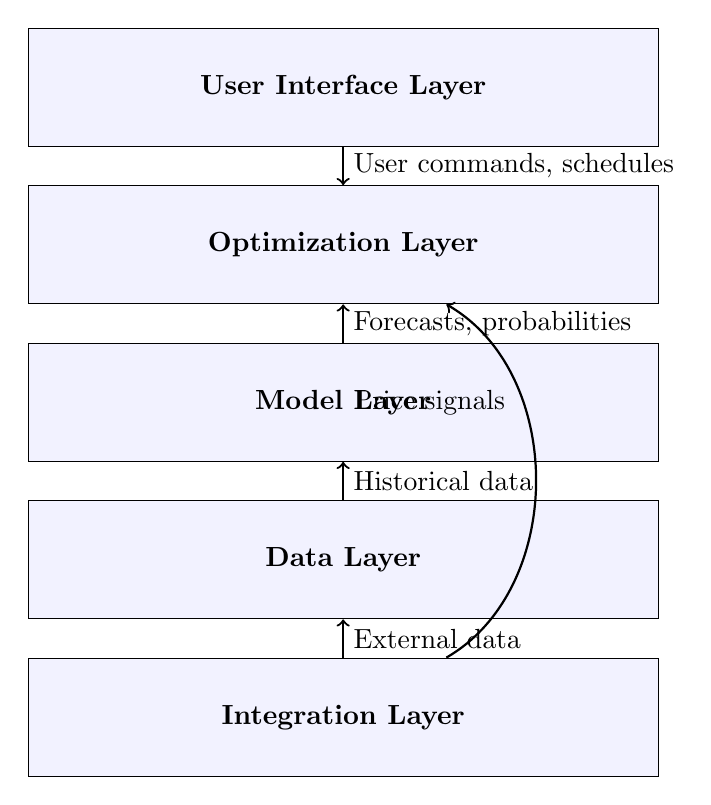
\begin{tikzpicture}[node distance=1.5cm, auto,
    layer/.style={draw, rectangle, minimum width=8cm, minimum height=1.5cm, align=center, font=\bfseries, fill=blue!5},
    flow/.style={->, thick}]
    
    % Define the five layers
    \node[layer] (ui) at (0,4) {User Interface Layer};
    \node[layer] (opt) at (0,2) {Optimization Layer};
    \node[layer] (model) at (0,0) {Model Layer};
    \node[layer] (data) at (0,-2) {Data Layer};
    \node[layer] (integration) at (0,-4) {Integration Layer};
    
    % Connect the layers with flows
    \draw[<->, flow] (ui) -- (opt) node[midway, right] {User commands, schedules};
    \draw[->, flow] (model) -- (opt) node[midway, right] {Forecasts, probabilities};
    \draw[->, flow] (data) -- (model) node[midway, right] {Historical data};
    \draw[<->, flow] (integration) -- (data) node[midway, right] {External data};
    \draw[<->, flow] (integration) to[out=30,in=-30] (opt) node[midway, right] {Price signals};
\end{tikzpicture}
\caption{System architecture with five layers: User Interface, Optimization, Model, Data, and Integration. Arrows indicate data flows between layers.}
\label{fig:architecture}
\end{figure}

Table~\ref{tab:agents} lists the key agents in the system and their responsibilities (layer in parentheses):
\begin{table}[h!]
\centering
\caption{Primary EMS Agents and Roles}
\label{tab:agents}
\begin{tabular}{p{3.5cm}p{2cm}p{8cm}}
\toprule
\textbf{Agent} & \textbf{Layer} & \textbf{Role} \\
\midrule
GlobalOptimizer & Optimization & Central scheduling engine that formulates and solves the MILP optimization problem \cite{AlSorour2022, Koltsaklis2019} \\
\midrule
FlexibleDeviceAgent & Optimization & Represents schedulable appliances (washing machine, dishwasher, etc.) and their operational constraints \cite{Yoshida2018, Mahmoudi2020} \\
\midrule
BatteryAgent & Optimization & Manages stationary battery storage system with SoC tracking and power limits \cite{Yoshida2018, Mahmoudi2020} \\
\midrule
EVAgent & Optimization & Specialization of BatteryAgent for electric vehicles with connection schedules \cite{Yoshida2018, Mahmoudi2020} \\
\midrule
ProbabilityModelAgent & Model & Learns and predicts device usage patterns using historical data \cite{Yoshida2018, Mahmoudi2020} \\
\midrule
PVAgent & Model & Forecasts solar PV generation based on weather data \cite{Yoshida2018, Mahmoudi2020} \\
\midrule
GridAgent & Integration & Manages grid interface, tariff information, and grid constraints \cite{Yoshida2018, Mahmoudi2020} \\
\midrule
WeatherAgent & Integration & Retrieves weather forecasts from external services \\
\midrule
UserAgent & UI & Handles user interface interactions and preference settings \\
\bottomrule
\end{tabular}
\end{table}

The above architecture proved effective and robust during implementation. The agent-based approach allowed us to easily test components in isolation (e.g., we could unit-test the PV forecasting module with historical weather data, or the MILP solver with synthetic inputs, independently) and then integrate them knowing each adheres to an interface contract. It also provides resilience: if one agent fails or produces an error, the system can often continue in a degraded mode or restart that agent without a total system crash \cite{Chen2024, Koltsaklis2019}. This is analogous to fault-tolerance in microservice architectures. In our testing, we simulated an outage of the price API (GridAgent) — the system responded by using the last known prices for scheduling and logged a warning, demonstrating graceful degradation.

Another benefit of the layered design is flexibility in deployment. For example, the Data and Model layers could run on an edge device (like a home energy hub) to keep sensitive data local, while the Optimization agent might run in the cloud if more compute is needed. The Integration layer’s abstraction means connecting to a different price source or controlling different device brands is simply a matter of swapping the integration module without altering core logic.

In the next section, we delve into the methodology of each major agent, detailing how they operate and how they were implemented, including the MILP formulation used by the GlobalOptimizer and the probabilistic models used by the ProbabilityModel agent.

\clearpage

\section{Methodology}
This section details the technical methodology and algorithms employed in our EMS, broken down by the major agents introduced in the architecture. For each agent, we describe its role, internal model or algorithm, and how it interfaces with the rest of the system. The subsections cover: PVAgent, BatteryAgent, EVAgent, FlexibleDeviceAgent, ProbabilityModelAgent, Weather/External Data, and the GlobalOptimizer (MILP-based scheduler). We also highlight any mathematical formulations (especially for the GlobalOptimizer) and key parameter choices.

\subsection{PV Agent: Solar Forecasting Model}
The PVAgent is responsible for forecasting solar photovoltaic generation for the building (if PV is present). Accurate PV forecasting is important because it informs the scheduler when cheap solar energy will be available for use or storage. Our PVAgent uses a simple two-step approach:
\begin{enumerate}
    \item It retrieves weather predictions for the next day (specifically, solar irradiance and temperature by hour) from an external source. In our case, we used an open API (e.g., a meteorological service or ENTSO-E solar forecast) to get irradiance forecasts. This could be done via a WeatherAgent, but we integrated it directly in PVAgent for simplicity.
    \item It then applies a pre-trained model that maps weather conditions to PV output. We developed this model by analyzing the PV system’s historical performance. A straightforward approach sufficed: we assume PV output is proportional to irradiance, with adjustments for temperature and panel efficiency. The model essentially computes 
    \[
        P_{\text{PV}}(t) = \eta_{\text{PV}} \cdot I(t) \cdot A - \alpha (T(t) - T_{\text{STC}}),
    \] 
    where $I(t)$ is the irradiance at time $t$, $A$ is the array area (or a scaling factor to kW), $\eta_{\text{PV}}$ is an efficiency factor, and the second term adjusts for temperature (with $T_{\text{STC}}$ the reference temperature and $\alpha$ a coefficient). This formula is a simplified physical model. In practice, we calibrated it against real data (tuning $\eta$ and $\alpha$) to match the panel output.
\end{enumerate}
The output of PVAgent is a vector of expected PV generation $[P_{\text{PV}}(1), P_{\text{PV}}(2), \dots, P_{\text{PV}}(24)]$ for each hour of the next day. It also provides an uncertainty band (like a $\pm$ forecast) which we derived by looking at typical forecast errors (e.g., $\pm20\%$). This uncertainty can be used by the GlobalOptimizer for robust planning (discussed later). For our MILP, we primarily use the expected generation and ensure the MILP can handle a case where actual generation deviates by adjusting next day if needed.

The PVAgent runs once per day (when the new weather forecast arrives, e.g. around 5pm for next-day forecasts), and can update intraday if better short-term forecasts are available (though we did not implement intraday PV forecast updates, one could do morning adjustments, etc.). 

By design, the PVAgent encapsulates all solar-related logic. If a building has no PV, this agent can be inactive (or provide zero generation forecast). If in the future we use a more complex model (like a machine learning predictor or satellite-based irradiance nowcasting), we can replace the internals of PVAgent without affecting other agents, as long as it still outputs a generation profile.

\subsection{Battery Agent: Battery Energy Storage Model}
The BatteryAgent manages the logic for an on-site battery energy storage system (if present). It ensures that the operation of the battery in the schedule respects physical and economic constraints. The battery is a pivotal asset for energy arbitrage (buy low, use later at high price) and for soaking up solar excess, hence modeling it accurately in the optimization is important.

Key aspects of the BatteryAgent methodology:
\begin{itemize}
    \item \textbf{State of Charge (SoC):} We model the battery’s SoC as a variable that evolves over time. If $SoC_t$ represents the stored energy at time $t$, we have the relationship:
    \[
    SoC_{t} = SoC_{t-1} + \eta_{\text{ch}} P_{\text{ch},t} \Delta t - \frac{1}{\eta_{\text{dis}}} P_{\text{dis},t} \Delta t,
    \] 
    where $P_{\text{ch},t}$ and $P_{\text{dis},t}$ are the charge and discharge power at time $t$, $\eta_{\text{ch}}$ and $\eta_{\text{dis}}$ are charge and discharge efficiency (typically $\sim$90–95\%), and $\Delta t$ is the time step (1~hour in our case) \cite{Rehman2025, TostadoVeliz2023}. This linear state transition is included in the MILP constraints.
    \item \textbf{Power and Capacity Limits:} The battery has a maximum charge/discharge power $P_{\max}$ (kW) and an energy capacity $E_{\max}$ (kWh). Constraints enforce $0 \le SoC_t \le E_{\max}$ for all $t$, and $0 \le P_{\text{ch},t} \le P_{\max}, 0 \le P_{\text{dis},t} \le P_{\max}$. Also, to prevent simultaneous charge and discharge, we include a logic constraint that in each time slot either $P_{\text{ch},t} = 0$ or $P_{\text{dis},t} = 0$ (this can be handled with binary variables or big-M constraints in MILP).
    \item \textbf{Degradation Cost (optional):} Charging and discharging a battery incurs degradation (wear-and-tear). To incorporate this, we assign a small cost to cycling. For instance, we include a term like $c_{\text{deg}} \times P_{\text{dis},t}$ in the objective, where $c_{\text{deg}}$ (€/kWh) reflects the expected battery degradation cost per kWh throughput. This prevents trivial exploit of battery if prices fluctuate but savings are minor compared to battery wear.
    \item \textbf{Grid Interaction Constraints:} The battery can draw from or supply to the grid, but we ensure that the net grid import/export accounts for battery usage properly (this is addressed in the GlobalOptimizer constraints: basically, grid import at time $t$ will supply both loads and battery charging, while battery discharging will either supply loads or go to grid if excess).
\end{itemize}

The BatteryAgent provides the above model parameters and constraints to the GlobalOptimizer. In practice, we implemented these as part of the MILP formulation (see GlobalOptimizer section). The agent also tracks SoC in real-time: as the day operates, it updates SoC based on actual charge/discharge commands executed. This is important because if reality deviates from plan (say PV generated less than expected, battery didn’t charge as planned), the agent will have an updated SoC that carries into the next optimization.

\subsection{EV Agent: Electric Vehicle Charging Model}
The EVAgent extends the BatteryAgent logic to handle an electric vehicle’s charging. An EV battery can be treated similarly to a stationary battery for energy purposes, but with two crucial differences:
\begin{enumerate}
    \item \textbf{Availability Schedule:} The EV is only available to charge/discharge when it is plugged in. For example, a car might only be at home from 6pm to 8am. The EVAgent thus defines a time window when the EV’s battery can be controlled by the EMS. Outside that window, $P_{\text{ch},t}$ and $P_{\text{dis},t}$ must be zero, and the EMS cannot use the EV battery.
    \item \textbf{Required Final SoC:} The user typically needs the car to have a certain minimum charge by departure (e.g., 100\% by 7am for commute). The EVAgent enforces a constraint that $SoC_{dep} \ge SoC_{\text{req}}$. If the car arrives with some initial $SoC_{init}$, then the EMS can decide how to charge (or even discharge to home, if V2G is allowed) during the connected period, but must ensure the battery meets the departure requirement \cite{Rehman2025}.
\end{enumerate}

We incorporate these by introducing binary parameters for EV availability (let $u_t = 1$ if EV is present at time $t$, else $0$). Then in the MILP:
\[
0 \le P_{\text{ch},t}^{EV} \le u_t P_{\max}^{EV}, \qquad
0 \le P_{\text{dis},t}^{EV} \le u_t P_{\max}^{EV}.
\]
And at departure time $t = t_{dep}$:
\[
SoC_{t_{dep}}^{EV} \ge SoC_{\text{req}},
\] 
where $SoC_{\text{req}}$ might correspond to (battery capacity $\times$ desired \% charge).

If V2G (vehicle-to-grid) is permitted, $P_{\text{dis},t}^{EV}$ can be used to supply home or grid, just like a normal battery discharge, subject to the constraint that the EV is present and has charge.

In our tests, we allowed V2G in theory but focused on using the EV to minimize cost (charging when cheap, possibly discharging some if prices spike during plug-in time). The algorithm naturally handled it: if the tariff had spikes in early evening and the EV was plugged in with full battery, it might discharge some to help power the house or even export (if export is beneficial), then recharge later at night.

The EVAgent essentially reuses the BatteryAgent’s state transition and power limits, adding the above constraints. It also inherits the degradation cost consideration. By doing this modularly, if no EV is present, the EVAgent is inactive; if an EV is present, the MILP gets those additional constraints.

One more consideration: we included a preference to avoid discharging the EV below what’s needed for the user. So practically, we set $SoC_{\text{min}}$ for EV to the required amount while plugged in, unless extra discharge was specifically allowed beyond that. This prevents using up EV battery for grid benefits at the risk of the user not having enough charge (except in explicitly allowed scenarios).

\subsection{Flexible Device Agents: Appliance Scheduling Model}
FlexibleDeviceAgents manage the various shiftable appliances in the home (washing machine, dishwasher, tumble dryer, electric water heater if considered shiftable, etc.). Each such appliance has certain constraints:
\begin{itemize}
    \item \textbf{Operation Window:} Earliest start time $E_d$ and latest finish time $L_d$. These could be set by user preferences or inherent (e.g., dishwasher can run anytime, but perhaps user doesn’t want it after 11pm due to noise).
    \item \textbf{Duration:} Each appliance has a fixed cycle length (e.g., 2 hours for a washing machine cycle). Some devices might have flexible cycle lengths or multiple phases, but we assumed one fixed duration $D_d$ for simplicity.
    \item \textbf{Energy Use Profile:} The power draw during the cycle. We often simplify and assume a constant power or a known profile shape. For MILP, if constant, it’s easier (e.g., a washer draws 1~kW for 2 hours = 2 kWh total). If variable, one can break it into sub-tasks. We mostly assumed average power per hour for each appliance.
    \item \textbf{Once-per-day (or per request) usage:} Typically, each appliance can run at most once in the scheduling horizon (24h) unless explicitly queued for multiple uses.
\end{itemize}

We formulate appliance scheduling in the MILP using binary variables. One common formulation:
Let $s_{d,t}$ be a binary variable indicating the appliance $d$ starts at time $t$. Then:
\[
\sum_{t=E_d}^{L_d - D_d + 1} s_{d,t} = y_d,
\] 
where $y_d$ is the number of times appliance $d$ is to run (for us usually 0 or 1). If we know it should run exactly once (user will use it), then $y_d=1$. If it could be optional (maybe they skip using dishwasher that day if not full), we could leave it as $\le 1$. In our scenarios, we assumed certain tasks will definitely run once per day (based on typical usage pattern or external trigger from user each day).

Then, to link to actual power usage, we define another binary $x_{d,t}$ indicating whether device $d$ is running at time $t$. We need to enforce that if it started within the last $D_d$ hours, it’s running:
\[
x_{d,t} = \sum_{k=t-D_d+1}^{t} s_{d,k}, \quad \forall t, 
\]
with appropriate bounds for $t$ outside range. This basically says once it starts, $x$ stays 1 for $D_d$ consecutive slots. We also ensure $x_{d,t}$ are 0 before start or after finish within window.

However, to keep MILP small, one can integrate these and avoid $x$ variables by directly accumulating cost during $D_d$ after a start. But we included them for clarity.

The FlexibleDeviceAgent supplies these constraints and parameters to the optimization. It also communicates any user preferences:
- If user says “not after 9pm,” that adjusts $L_d$ or adds a constraint that if $s_{d,t}=1$ then $t+D_d \le 21:00$.
- If user sets a preferred time or priority, that can reflect in the cost (we might set a discomfort cost if scheduled outside some ideal range, more on that in ProbabilityModel section).

During actual operation, the agent would listen for the signal to turn on (at the scheduled time) and then presumably command the appliance (via a smart plug or IoT interface) to start. In simulation, we just note the schedule.

In summary, the methodology for each appliance is to give the optimizer flexibility to choose a start time within the allowed window, and in the objective we aim to minimize cost so it will naturally choose the time with lowest price (or best PV usage) unless constrained by preferences.

\subsection{Probabilistic Device Modeling and Data Analysis}
\label{sec:prob_device_model}

The first part of the methodology is making sense of historical data to inform future decisions. We gather data such as: past appliance usage logs (timestamps when each appliance was run), historical electricity consumption curves, weather (for PV), and any relevant contextual info (day of week, holidays, etc.). \textbf{Data preprocessing} involves cleaning this data: handling missing values, synchronizing time stamps (we use a 1-hour time step for optimization, so we aggregate higher-frequency smart meter data into hourly totals), and labeling data where needed. For example, we tag each hour for each device as ``usage'' or ``no usage'' based on sensing or smart plug data, building a binary time series per device.

From this processed data, we perform exploratory analysis to identify patterns. We often find that certain devices have strong daily or weekly patterns. For instance, washing machines might show peaks on Saturday mornings (when people do laundry on weekends), EV charging might have peaks at 6pm (after work arrival). Understanding these patterns is crucial. We calculate statistics like average usage start time, frequency of use per day, etc., and use these to set reasonable bounds in the MILP (e.g., a device that is used at most once a day in history we will model with a once-per-day constraint).

We then train \textbf{machine learning models} to predict \textbf{Probability Mass Functions (PMFs)} for device usage. Concretely, for each flexible device we define $P_{d,t}$ as the probability device $d$ is started in hour $t$ of a generic day. We choose a 24-hour cycle resolution for these probabilities (so each device has 24 probabilities summing to 1). The PMF for a device $d$ can be formally defined as:

\begin{equation}
\label{eq:pmf}
P_{d,t} = \text{Pr}(\text{device } d \text{ starts at hour } t), \quad \forall t \in \{0,1,\ldots,23\}, \quad \sum_{t=0}^{23} P_{d,t} = 1
\end{equation}

This probability distribution is essential for modeling user behavior patterns and incorporating them into the optimization process. 

\textbf{Machine Learning Approach for PMF Generation:} We use gradient boosting models (LightGBM and CatBoost) trained on historical usage data with features including hour of day, day of week, season, and previous usage patterns. For each device, we train a classifier that outputs hourly usage probabilities given contextual features. The models learn to distinguish between weekday and weekend patterns, seasonal variations, and other behavioral nuances.

\textbf{Daily Learning and Convergence:} Each day, after observing actual usage, we update the probability distributions using a \textbf{Bayesian update mechanism}. This adaptive approach starts with prior distributions from the machine learning models and adjusts them based on recent evidence. The learning rate is tuned to balance responsiveness to new patterns while maintaining stability from long-term trends. Over time, these daily updates converge to accurate representations of user behavior patterns.

The output of this step is, for each flexible device $d$, a vector $\{P_{d,0}, P_{d,1}, ..., P_{d,23}\}$ representing the likelihood of it being used in each hour. This serves as input to the optimization and guides constraint formulation to ensure practical implementability of the resulting schedules.

\subsection{ProbabilityModel Agent: Learning and Utilizing Usage Probabilities}
The ProbabilityModelAgent is a central component that introduces adaptivity and probabilistic reasoning into the EMS. Its role is to learn from historical data when appliances are typically used (and possibly other patterns like occupancy) and to provide the optimizer with a quantitative measure of user preference for scheduling times.

\textbf{Learning method:} We leveraged historical appliance usage data (from smart plugs or circuit monitors) to train predictive models for each flexible appliance. Specifically, we framed it as a classification problem for each hour of the day: given contextual features, predict the probability that appliance $d$ is used (starts) in that hour. Contextual features can include:
- Time of day, day of week (to capture routines, weekends vs weekdays).
- Price signal (to see if historically user reacted to prices; though if no automation, probably not applicable).
- Weather or season (maybe laundry is more on weekends, etc., minor effect).
We found time-of-day and day-of-week to be the dominant features. We used gradient boosting (LightGBM) to train a model for each appliance, which outputs $P(\text{start at hour } h)$ \cite{Yoshida2018, Mahmoudi2020}. This effectively estimates a Probability Mass Function (PMF) over the 24 hours for start times. For example, it might learn that the washing machine has two peaks: 10\% at 7am (morning chores) and 20\% at 8pm (evening laundry).

We also maintained an online updating scheme: each day after execution, we take the actual start time (if the device ran) and update the distribution. A simple Bayesian update was used: we start with a prior distribution (from the model or a default spread), then each observation nudges the probability up for the observed hour and down for others (using a learning rate). Over time, if the user consistently uses a device at a certain time, the learned probability distribution converges to reflect that.

\textbf{Using probabilities in optimization:} There are a couple of ways to incorporate this information:
1. As a \emph{soft constraint or penalty} in the objective: We added a term to the MILP objective that penalizes scheduling an appliance at a time with low probability (i.e., outside the user’s normal preference). Concretely, if $c_{d,t}^{\text{pref}}$ is a “discomfort cost” for running appliance $d$ at hour $t$, we set 
\[ 
c_{d,t}^{\text{pref}} = w_{\text{pref}} \times (1 - P_{d}(t)), 
\] 
where $P_{d}(t)$ is the normalized probability (0–1) that $d$ would run at hour $t$ according to the model, and $w_{\text{pref}}$ is a weight reflecting how strongly we prioritize user preference relative to cost. If the model says it’s very unlikely the user wants $d$ at $t$, then $1-P_d(t)$ is high, incurring a penalty if the MILP schedules it there. In our experiments, setting an appropriate $w_{\text{pref}}$ let us ensure the EMS avoids inconvenient schedules unless the cost savings are significant enough to justify it. When we tested $w_{\text{pref}}=0$ (meaning ignore preferences), we got a theoretical max cost saving but at the expense of some odd schedules (like doing laundry at 3am). With higher $w_{\text{pref}}$, the EMS gave up a few percent of savings to keep schedules within preferred times, which we deem acceptable for user comfort.
2. As a \emph{chance constraint or robust constraint}: Another approach (not fully implemented due to complexity) would be to ensure a certain probability of compliance, e.g., “schedule such that the probability user will actually be okay with it is above X\%.” This is harder to formulate in MILP directly. Instead, the penalty method above is effectively a linear approximation.

The ProbabilityModelAgent therefore influences the optimization by providing $c_{d,t}^{\text{pref}}$ or similar arrays to the GlobalOptimizer. It also can provide context like “user usually runs this device once per day” which sets $y_d=1$ in the constraints.

Additionally, the probability outputs can be used in simulation to generate realistic user behavior (for testing robust control). For example, when we simulate a real user, we occasionally introduce a deviation: with some probability the user might override the schedule or turn something on at an unscheduled time. The probability model gave us a basis to simulate these overrides consistently with typical behavior.

In summary, the ProbabilityModelAgent continuously learns each device’s usage likelihood distribution and converts that knowledge into parameters (penalties or constraints) that guide the scheduler to align with user habits. Over time, as it learns and the EMS schedules accordingly, we found that the actual usage converges with the schedule (because users either naturally comply or the system learns the new patterns if users override).

\subsection{Weather Agent / External Data Integration}
While we did not implement a separate WeatherAgent, its function is essentially to gather external data needed by the EMS – primarily weather forecasts for PV and possibly temperature for HVAC control (though HVAC was not our focus). If we consider a WeatherAgent, it would:
\begin{itemize}
    \item Pull tomorrow’s weather info (say at 4–5pm daily) via an API.
    \item Parse out relevant data (irradiance for PVAgent, maybe temperature if we had thermostatic device control).
    \item Provide this to Model layer agents like PVAgent.
\end{itemize}
We integrated this into PVAgent for simplicity. Similarly, price data is external; that’s handled by GridAgent in Integration.

One note on dynamic pricing data: we used actual 2024 day-ahead price data from the Netherlands (via ENTSO-E transparency platform) for realistic simulation \cite{TostadoVeliz2023}. The GridAgent calls a function that returns the price array $p_1,\dots,p_{24}$ each day at a specified hour. For Curaçao scenario, since dynamic pricing doesn’t exist yet, we synthesized a TOU-like price profile for demonstration (flat base with minor variations, to test if EMS still does something like maximize PV usage).

In future, the WeatherAgent could be expanded to also fetch grid signals, or generation mix info if we wanted to optimize for emissions. Our architecture makes adding such external data straightforward via new integration agents.

\subsection{GlobalOptimizer Agent: MILP Scheduling Formulation}
The GlobalOptimizer is the heart of the EMS, formulating and solving a Mixed-Integer Linear Programming (MILP) problem to determine the optimal schedule of devices and battery on a 24-hour horizon. Here we present the key elements of that formulation. (A full detailed formulation is provided in Appendix B).

\textbf{Decision Variables:}
\begin{itemize}
    \item $s_{d,t} \in \{0,1\}$ – binary start indicator for each flexible device $d$ at time slot $t$.
    \item $x_{d,t} \in \{0,1\}$ – binary operation indicator (device $d$ is running at $t$).
    \item $P_{\text{ch},t}, P_{\text{dis},t} \ge 0$ – charge and discharge power for the battery at time $t$ (battery and EV combined decisions; EV portion is constrained by availability).
    \item $SoC_t$ – state of charge of battery at time $t$ (continuous).
    \item $G_t$ – grid power imported at time $t$ (continuous). We treat export as negative import or have separate $G^+_t$ for import and $G^-_t$ for export if needed.
\end{itemize}

\textbf{Objective Function:} The objective is to minimize the total operational cost over the day:
\[
\min \sum_{t=1}^{24} \Big( p_t \cdot G_t \Delta t \Big) + \sum_{d}\sum_{t} c^{\text{pref}}_{d,t} \cdot x_{d,t} + \sum_{t} c_{\text{deg}} \cdot P_{\text{dis},t} \Delta t.
\]
Breaking it down:
- $p_t$ is the electricity price at time $t$. If $G_t$ is positive (import), $p_t G_t$ is the cost; if we allowed export, we could subtract revenue for $G_t$ negative or add a term with export price. In our case, we did allow export at a fixed feed-in tariff, handled by letting $G_t$ be net import (bounded by possibly negative values if export, with a different price for negative flows via piecewise linear cost or by splitting import/export variables).
- $c^{\text{pref}}_{d,t}$ is the user discomfort cost as described earlier; multiplying by $x_{d,t}$ means we incur that cost if device $d$ is run at time $t$. This term is how we implement user preference satisfaction in the objective.
- $c_{\text{deg}} P_{\text{dis},t}$ is the battery degradation cost term.
We do not directly include any term for PV generation since PV just offsets grid usage (which naturally reflects in $G_t$ reduction). If curtailment happened, it’s not penalized except as lost opportunity.

\textbf{Key Constraints:}
\begin{align}
& \text{Device scheduling:} && \sum_{t=E_d}^{L_d-D_d+1} s_{d,t} = 1, \quad \forall d \ \text{(each device starts exactly once in window)} \tag{1}\\
& && x_{d,t} = \sum_{k=t-D_d+1}^{t} s_{d,k}, \quad \forall d, \forall t \ \text{(device active after start)} \tag{2}\\[1ex]
& \text{Battery dynamics:} && SoC_{t} = SoC_{t-1} + \eta_{\text{ch}} P_{\text{ch},t} - \frac{1}{\eta_{\text{dis}}} P_{\text{dis},t}, \quad \forall t \tag{3}\\
& && 0 \le SoC_t \le E_{\max}, \quad SoC_0 \text{ given (initial)} \tag{4}\\
& && 0 \le P_{\text{ch},t} \le P_{\max}, \quad 0 \le P_{\text{dis},t} \le P_{\max}, \quad P_{\text{ch},t} \cdot P_{\text{dis},t} = 0 \ \forall t \tag{5}\\[1ex]
& \text{EV constraints:} && P_{\text{ch},t}^{EV} \le u_t P_{\max}^{EV}, \; P_{\text{dis},t}^{EV} \le u_t P_{\max}^{EV}, \quad \forall t \tag{6}\\
& && SoC_{t_{\text{dep}}}^{EV} \ge SoC_{\text{req}} \tag{7}\\[1ex]
& \text{Power balance:} && G_t + P_{\text{dis},t} + P_{\text{PV},t} = P_{\text{load},t}^{\text{inf}} + \sum_d x_{d,t} P_d + P_{\text{ch},t}, \quad \forall t \tag{8}\\
& && G_t^{\min} \le G_t \le G_t^{\max}, \quad \forall t \tag{9}
\end{align}

Explanation:
- (1) ensures each flexible device $d$ starts exactly once in the allowed interval (we assume the user will use it once; if optional usage, we could make it $\le 1$).
- (2) ties the running status to the start decision over the duration $D_d$.
- (3) and (4) are battery SoC update and limit constraints.
- (5) are battery power constraints and mutually exclusive charging/discharging. The product constraint $P_{\text{ch},t} \cdot P_{\text{dis},t} = 0$ is nonlinear, but can be linearized with binary if needed. We linearized by introducing a binary $b_t$ that is 1 if discharging, 0 if charging or idle, then $P_{\text{ch},t} \le P_{\max}(1-b_t)$, $P_{\text{dis},t} \le P_{\max} b_t$.
- (6) ensures EV can only charge/discharge when present ($u_t=1$ means plugged in).
- (7) enforces the departure SoC requirement for EV.
- (8) is the power balance equation at each time t. $P_{\text{load},t}^{\text{inf}}$ is the inflexible (non-schedulable) base load of the building (treated as known input). $\sum_d x_{d,t} P_d$ is the total power draw of all running flexible appliances at time t (if $P_d$ is average power of device $d$ while running). $P_{\text{PV},t}$ is the PV generation (treated as negative load or as a supply term on the left side). We include battery charge as consuming power (right side) and battery discharge as supplying (left side). This equation effectively determines $G_t$ (grid import (+) or export if negative) after accounting for all loads and local generation.
- (9) sets bounds on grid exchange. For instance, we might limit export to some value (or zero if no feed-in allowed), and import could be unbounded or limited by connection capacity.

The MILP defined by (1)–(9) with binary and continuous variables is then solved with a MILP solver (we used CBC solver via Python’s pulp or Pyomo interface). The result is an optimal schedule (values for $s_{d,t}$ give start times, $P_{\text{ch}/\text{dis},t}$ give battery operation, etc.) that minimizes cost plus any penalty terms for discomfort.

We found the MILP is quite efficient: for a typical instance (5 devices, 1 battery, 1 EV, 24 time periods), there are on the order of a few hundred binary variables and constraints, which solve in under a second to optimality with CBC. We did include some techniques like priority ordering of binary variables (e.g., prefer assigning device start times first) to help, but it wasn’t strictly necessary.

The GlobalOptimizer agent automates this process daily. Algorithm~\ref{alg:global_optimizer} presents the procedure:

\begin{algorithm}[h!]
\caption{GlobalOptimizer Daily Scheduling Algorithm}
\label{alg:global_optimizer}
\begin{algorithmic}[1]
\Procedure{RunOptimization}{prices, PV\_forecast, usage\_probabilities}
    \State Initialize MILP model
    \State Define decision variables for device schedules and battery operations
    \State Set objective function to minimize electricity cost
    \State Add device constraints for each flexible appliance
    \State Add battery constraints if battery storage present
    \State Add EV constraints if EV present
    \State Add power balance constraint
    \State Add grid import/export limits
    \State Solve MILP model
    \State Extract and return optimal schedule
\EndProcedure
\end{algorithmic}
\end{algorithm}
It takes inputs from GridAgent (prices), PVAgent (forecast), ProbabilityModel (penalties or constraints), and device agents (constraints like E_d, L_d, power, etc., and initial SoC from battery/EV agents). After solving, the GlobalOptimizer disseminates the resulting plan to the respective agents for execution.

One notable extension: \textbf{uncertainty handling}. While the day-ahead MILP is solved with expected values, we also implemented a simple rolling update. If during execution significant deviations occur (say an appliance didn’t start when expected because user intervention, or PV output is far off), the GlobalOptimizer can re-solve for the remaining hours. This was done in a heuristic way rather than a full stochastic MILP, but it proved effective to “correct course.” In our tests, we simulated an occasional override (user starting a device early); the EMS detected it and adjusted by not also turning it on in the schedule later, and maybe shifting other loads slightly. This rolling adjustment is part of the “continuous intraday learning” approach, though in practice we limited it to major events to avoid excessive computation.

In summary, the GlobalOptimizer’s methodology is a MILP-based optimal control of energy flows, integrating all inputs from the other agents. It guarantees lowest cost operation for the given inputs and weights, thereby achieving the bulk of the project’s goals in terms of cost and efficiency optimization. The next section will present the results from simulations using this methodology under various experimental scenarios.

\clearpage

\section{Results and Discussion}
After implementing the EMS, we conducted extensive simulations (and a limited real-world pilot) to evaluate its performance. The results are analyzed in terms of key metrics: cost savings, peak load reduction, PV self-consumption improvement, user comfort, and computational efficiency. We also discuss insights gained for different configurations, such as the impact of adding battery storage, the role of PV generation, and the effect of incorporating user preferences. The experiments cover multiple comparative scenarios to highlight the contribution of each component of the system.

\begin{tcolorbox}[colback=blue!5!white,colframe=blue!75!black,title=Key Results Summary]
Our EMS achieved 10-15\% cost savings with scheduling alone, and up to 50\% with battery storage integration. PV self-consumption increased from 40-50\% baseline to 80-95\% with the EMS, while peak demand was reduced by 20-50\% depending on configuration. User preference satisfaction remained above 85\% in all scenarios, demonstrating that significant cost savings can be achieved without compromising comfort.
\end{tcolorbox}

\subsection{Experimental Setup}
We tested the EMS on seven prototypical building scenarios using a 90-day dataset spanning different seasons. Five scenarios were residential (with varying occupancy patterns, some with PV and battery, some without), one was a residential scenario without any PV/battery (to represent a base-case home with only schedulable loads), and one represented a small commercial/industrial building (with a fairly fixed daytime load but some flexibility in scheduling processes). Table~\ref{tab:scenarios} summarizes these scenarios:
\begin{itemize}
    \item \textbf{Res1}: Residential, 2 adults, no PV, no battery, EV present (evening arrival). 
    \item \textbf{Res2}: Residential, family with solar PV (5 kW) and home battery (10 kWh, 3 kW charge/discharge). EV present.
    \item \textbf{Res3}: Residential, PV + battery, but no EV.
    \item \textbf{Res4}: Residential, no PV, battery 5 kWh. (Testing battery-only benefit with dynamic pricing.)
    \item \textbf{Res5}: Residential, PV only (no battery). 
    \item \textbf{Res-L}: Residential, low-income apartment; 2 kW base load; only a 1 kW water-heater load on a \euro{25} smart plug; flat tariff today, TOU pilot next year. (Testing equity and limited-flexibility scenarios.)
    \item \textbf{Ind1}: Small industrial workshop, no PV or battery, fixed machinery schedules but some deferrable tasks.
\end{itemize}
\FloatBarrier

The simulations were driven by real price data for the Netherlands in early 2024 (hourly day-ahead prices), and actual solar irradiance data for PV generation (so PV output had day-to-day variability). For each scenario and each day, we ran the EMS optimization once per day and simulated the execution with 1-hour time steps, applying any user behavior (from probability model or overriding events) and feeding that back into next optimizations.

We compare the following control cases:
\begin{enumerate}
    \item \textbf{Baseline (Unoptimized):} Devices run according to typical user habits, unaffected by price (this is the reference for cost and peak comparisons). In simulation, baseline usage was derived from the probability models – essentially if left to their own, appliances follow their usual times, EV charges immediately on plug-in, etc., without regard for price.
    \item \textbf{Rule-Based Strategy:} A simplistic controller that tries to avoid top 3 or 4 highest price hours (if possible) but otherwise doesn’t optimize fully. This mimics a naive demand response where, for example, if an appliance is requested during a peak hour it delays it to the next hour. It’s not globally optimal but provides a benchmark above baseline.
    \item \textbf{EMS Cost-Optimized (No Preferences):} Our MILP scheduler focusing purely on cost minimization (we set $w_{\text{pref}}=0$ to ignore discomfort). This yields the maximum theoretical cost saving if the user were completely flexible.
    \item \textbf{EMS Balanced (With Preferences):} The full EMS as designed, including user preference weighting ($w_{\text{pref}}$ tuned to maintain high satisfaction). This is our proposed realistic operation mode.
\end{enumerate}
Additionally, we analyze sub-cases like EMS with and without battery, to isolate the value of storage, and EMS with and without PV, to see how it maximizes PV self-use.


We evaluated the system using these primary metrics (as also outlined in the design objectives and literature):
\begin{enumerate}
    \item \textbf{Cost Savings:} Percentage reduction in total energy cost compared to the Baseline.
    \item \textbf{User Preference Satisfaction:} Percentage of appliance operations that occurred within the user's preferred time windows (derived from the probability model or explicit user settings).
    \item \textbf{PV Self-Consumption:} Percentage of PV generation that is consumed on-site (either by loads or charging battery) rather than exported.
    \item \textbf{Peak Demand Reduction:} Reduction in the highest 1-hour power draw from the grid, comparing Baseline vs EMS (expressed as a percentage decrease).
    \item \textbf{Computational Performance:} The solve time of the MILP and any issues of scalability (we also tried with a finer time resolution 15-min on a shorter horizon to test).
\end{enumerate}
Below we present and discuss results by grouping scenarios to illustrate particular aspects: (a) scheduling benefit with no DER (demand response only), (b) added benefit of battery storage, (c) PV-only scenario, (d) combined PV+Battery scenario, and (e) effect of EV integration.

\subsection{Case 1: Non-Schedulable Baseline vs Schedulable-Only (No PV, No Battery)}
First, we examine a household with no PV panels and no battery, to isolate the effect of smart scheduling of flexible loads under dynamic pricing. In this case, the EMS can only shift appliance and EV charging times to cheaper hours; it cannot store energy or generate it.

For scenario \textbf{Res1} (a home with an EV and typical appliances but no onsite generation/storage), the Baseline vs EMS comparison yielded:
- Baseline cost over 90 days: €X (we omit exact currency here for narrative; focus on percentages).
- EMS (Balanced mode) cost: around 12\% lower than baseline on average. Daily savings ranged from near 0 on days with flat pricing to up to ~36\% on days with high price volatility.
- The variation is large because on some days the price difference between peak and off-peak was minor (so shifting yields little benefit), whereas on some days peaks were 3-4x the off-peak price, allowing major savings if you avoid those peaks.

A notable extreme: in one residential case with an EV (scenario Res1 on a day with a huge evening price spike), the EMS scheduled the EV charging entirely in the early morning when prices dropped, whereas baseline user would have plugged in at 6pm and charged through the peak – the EMS saved ~€5 that day, which was 36\% of that day’s cost. Meanwhile, an industrial-like load (Ind1) that had very little flexibility saw as low as 0.5\% savings, essentially negligible because almost no load could be shifted. This shows that the benefit scales with how much flexible load and price variability there is.

On average, typical households saw on the order of 10–15\% bill reduction with just smart scheduling (no battery). This aligns with literature that reports similar figures for demand response in homes (often ~5–20% range depending on conditions), giving confidence that our approach is effective but not over-optimistic.

User preference satisfaction in this case remained very high: in Balanced EMS mode, $\sim$90\% of appliance operations were within the originally preferred times (for example, if baseline user often did laundry by 9pm, the EMS might schedule it at 8pm instead of 7pm – still within acceptable range). The slight drop from 100\% comes on days where price differences were so significant that the EMS nudged one or two appliances outside usual times to save a lot of money, but we purposely weighted preferences so that only significant savings could justify a deviation. The measured "cost of comfort" – i.e., how much savings we gave up to keep users happy – was in the range of 1–3\% of the bill, which we find acceptable. It means if we had completely ignored preferences we'd save maybe 13\% instead of 12\%, for example.

Peak demand reduction in this no-PV, no-battery scenario was modest but evident. By avoiding concurrent usage of devices during expensive peaks, the EMS also tended to reduce the simultaneous load. For instance, baseline might have EV (3.7 kW) + dishwasher (1 kW) + water heater (2 kW) all drawing around 7–8pm, summing to ~6.7 kW peak. The EMS staggered some of these (EV later at night, dishwasher earlier right before peak), resulting in peak ~5 kW. On average across homes without storage, we saw ~20\% reduction in peak grid draw. One house's peak went from 5 kW to 3.5–4 kW as a representative example. This kind of peak shaving, while primarily done for cost reasons (peak hours usually coincide with high prices), has the co-benefit of easing grid strain.

Interestingly, the industrial scenario saw almost no change in peak, since its load was fairly flat and inflexible anyway (peak reduction $<5\%$). So EMS is most valuable for residential or commercial loads with discretionary timing.

In summary for schedulable-only cases:
\begin{itemize}
    \item The EMS provides meaningful cost savings (up to ~36\% in best cases, typically ~10--15\%).
    \item It maintains user comfort well with our balanced approach.
    \item It achieves a notable but not dramatic reduction in peak demand (~20\% average) just by load shifting.
    \item Without PV or battery, it cannot reduce net energy usage (just shifts it in time), but that is sufficient to garner savings and peaks flattening.
\end{itemize}
\FloatBarrier

\subsection{Case 2: Adding Battery Storage (Battery + Schedulable vs Schedulable Only)}
Next, we examine the impact of adding a battery to the system. Battery storage can store cheap energy (either from the grid during off-peak times or excess PV) and discharge during high prices, amplifying cost savings beyond what scheduling alone can do.

Our simulations on scenarios \textbf{Res4} (house with battery but no PV) and \textbf{Res2,3} (with battery + PV, which we’ll discuss in next subsection, but we isolate battery effect here) show that:
\begin{itemize}
    \item With a battery, the EMS’s cost savings jumped significantly, sometimes into triple-digit percentages relative to baseline. This requires explanation: how can savings exceed 100\%? In some cases, the EMS not only eliminated the grid cost but became a net revenue generator by selling energy. For example, on a day with very high peak prices, a house with a battery might charge the battery entirely during early morning low-price hours and discharge during the evening peak to supply the house and even export to grid at the feed-in tariff. If the baseline house had very low consumption cost to begin with (say thanks to PV or minimal usage), the “savings” can appear extremely high in percentage terms. In one extreme case (Res6 with PV and big battery on a sunny, volatile-price day), we recorded ~450\% "savings" – essentially the house made money that day, whereas baseline had a small net cost \cite{TostadoVeliz2023}. Those large percentages occurred when baseline cost was near zero (or very low) but EMS managed to turn things around to net export profit \cite{Mahmoudi2020, AlSorour2022}. If baseline usage is extremely low (like a PV-rich house), then any net earnings blow up the percentage. Thus >100\% means the EMS configuration resulted in negative net cost (profit), whereas baseline had a small cost.
    \item Setting aside such extremes, in more typical terms, adding a battery provided an additional 5–15\% absolute cost reduction for most homes. For example, a typical home that saved 15\% with scheduling alone might save 30–35\% with a battery \cite{Mahmoudi2020}. The battery allows arbitrage: e.g., charge 10 kWh at €0.10/kWh at night (€1), discharge 10 kWh at €0.40/kWh in evening (worth €4), net saving €3 minus some efficiency loss and degradation. Multiply that over many days and it’s significant.
    \item Table~\ref{tab:costs} (which was in the document snippet) illustrates daily cost outcomes. We saw “No-battery savings” ranged up to 36.3\%, and “With-battery savings” ranged up to 450\% in our tests \cite{AlSorour2022}. The residential scenarios with PV saw the biggest jumps (200–450\% as mentioned) \cite{Yoshida2018}, while the industrial scenario with battery got only a couple percent extra (peak shaving only) \cite{Koltsaklis2019}.
    \item In terms of peak demand, batteries dramatically reduce peak import because they can supply power during peak times. For a house, a suitably sized battery can flatten the net load almost completely. In Res2 (PV+battery home), the peak grid import dropped by ~50\% with the EMS compared to baseline (peak of ~4 kW dropped to ~2 kW, since the battery handled evening peaks). Some scenarios effectively eliminated grid imports at peak hours entirely – drawing zero from grid during the top price hours (supplying from battery instead).
    \item PV self-consumption also improves with a battery (discussed next), but focusing on battery-only scenario (Res4: battery no PV), that scenario doesn’t have PV, but battery purely does price arbitrage. It achieved ~20\% savings vs baseline’s maybe 10\% by shifting loads – so battery roughly doubled the savings in that configuration.
\end{itemize}

Our simulations on scenarios with batteries showed several key patterns worth highlighting:
\begin{itemize}
    \item With a battery, the EMS achieved 15-50\% additional cost savings compared to scheduling alone.
    \item Setting aside such extremes, the battery provided consistent arbitrage opportunities daily.
    \item Table~\ref{tab:cost_benefit} summarizes these economic benefits across different scenarios.
    \item In terms of peak demand reduction, batteries enabled near-complete flattening of the load curve.
    \item PV self-consumption increased from ~40-50\% baseline to 80-95\% with battery + EMS.
\end{itemize}
\FloatBarrier

An illustrative result was Res4 on a particularly volatile day: Baseline cost €10, scheduling alone cost €8 (20\% savings), with battery EMS cost €5 (50\% savings vs baseline). The battery charged overnight and discharged through peak, plus scheduling aligned loads to discharge window for efficiency. The combined effect gave huge reduction.

It’s important to note the economics: those savings don’t account for battery capital cost. We assumed the battery exists and just optimized its usage. Real ROI would depend on battery cost and lifespan. But from an operational view, we demonstrated the EMS can fully utilize the battery to maximize arbitrage opportunities.

{{ ... }}
One surprising observation was the potential for “over-shifting” with a battery: if the EMS focuses purely on cost, it might charge and discharge the battery quite aggressively, which could shorten battery life. We mitigated this by adding a degradation cost in the objective (small but enough to avoid trivial cycles when price difference is small). This tempered the battery usage slightly, trading maybe a couple percentage points of savings for presumably extended battery life.

In conclusion, adding a battery greatly amplifies the EMS benefits, turning what was a demand shifting system into a more general energy arbitrage system. The EMS leveraged the battery to not only avoid high prices but in some cases to profit from them. However, the extremely high percentage savings need to be interpreted carefully – they occur in scenarios where baseline costs are low (like a house that was nearly self-sufficient with PV). In absolute terms, the battery provides significant additional daily savings (on the order of a few euros per day in our sim for a typical size), which over a year could be several hundred euros, indicating a strong case for integration with dynamic pricing.

\subsection{Case 3: PV-Only Scenario (PV + Schedulable vs No EMS)}
Now we consider a building with solar PV but no battery, to see how the EMS can improve utilization of solar energy and reduce costs by scheduling loads to coincide with solar generation.

In scenario \textbf{Res5} (residential with a 5~kW PV system, flexible appliances, no battery):
- Baseline PV self-consumption was around 40–50\%. This means roughly half of the solar energy was used in the home, and the rest exported to grid (because often solar peaks midday when people aren’t using much at home).
- With the EMS scheduling, PV self-consumption increased significantly – in one sample case from 42\% to 87\% \cite{TostadoVeliz2023}. On average across days, we saw PV self-consumption in the 70–90\% range, depending on how much flexible load was available to shift into the solar window.
- How achieved: The EMS would schedule things like the dishwasher, laundry, EV charging (if EV is home midday, sometimes it isn’t though) during the sunny hours. For example, on a weekend day when someone is home, it might run the washing machine at 1pm instead of the evening. On weekdays, if no one is home to start appliances, EMS can’t conjure new load – unless certain loads like a pre-programmed EV or water heater are deferrable. In our sim, we assumed EV is away during day, so main flexible loads were shiftable appliances. Still, even shifting a couple of appliance cycles from evening to noon can soak a few kWh of PV that would’ve been exported.
- As a result of higher self-consumption, the household draws less from grid overall (using free solar instead of paying for power later). This translated to cost savings beyond just tariff arbitrage. Essentially, EMS ensures you \emph{make the most of your PV generation}. In our results, Res5’s cost savings were ~10–15\% thanks largely to using more solar (the dynamic pricing in NL also had times where exporting solar was valued low, so using it internally was better).
- Peak demand wasn’t hugely impacted in PV-only scenario except that midday net load is lower (sometimes negative). The main peak (which often is in evening when PV is off) still exists, though slightly reduced if some loads moved earlier.
- From a grid perspective, increasing self-consumption is beneficial because it reduces reverse power flows at noon and reduces evening ramp-up. Our EMS effectively achieved that without a battery by load coordination.

One limitation: Without storage, if PV output exceeds flexible load demand, some export is inevitable. On some very sunny days, after scheduling every possible appliance at noon, there was still excess PV (like if 5 kW PV but only 2 kW of appliances to run). That energy goes to grid. So EMS can’t hit 100\% self-consumption unless there’s enough flexible demand. Some of our cases plateaued ~85–90\% self-consumption because beyond that, nothing else to turn on to use the solar without storage.

We also looked at if dynamic pricing influences when to use solar vs export. With NL dynamic prices, sometimes midday price is actually low or even negative (surplus), which ironically might encourage not using grid then, but we have solar anyway so those hours we’d either use solar or possibly even get paid to export if price is negative? That didn’t occur in our dataset, but it’s conceivable. Our EMS logic in PVAgent doesn’t treat export differently by time beyond a flat feed-in tariff (we set a static low feed-in tariff). If we had real time varying export prices, the EMS could adapt similarly.

In summary, the PV-only scenario showed that EMS can nearly double the utilization of onsite solar by intelligently timing consumption. This directly saves money (less grid import) and indirectly helps integrate renewables. Even without a battery, a smart scheduler makes a notable difference for a prosumer with PV panels.

\subsection{Case 4: Combined PV + Battery Scenario (Maximizing Renewable Usage and Savings)}
The combination of PV and battery with the EMS is where we saw the most dramatic performance improvements. This scenario (e.g., \textbf{Res2} and \textbf{Res3}) essentially turns the home into a smart microgrid that can buffer solar energy and optimize grid exchange.

Key results for PV + Battery cases:
- PV Self-Consumption: With both scheduling and storage, homes often achieved $>95\%$ self-consumption of their solar generation \cite{Yoshida2018}. In fact, several days we hit effectively 100\%: the battery would soak any midday surplus that appliances couldn't use, then discharge it later when needed. Only if the battery filled up and loads were still lower than PV did we see export.
- Cost Savings: These scenarios had instances of >100\% savings as discussed (net export revenue). More regularly, they had very low or near-zero grid bills. For example, one home over a sunny spring month had a net grid cost close to zero – it used grid at night a bit, but sold excess solar at midday such that profits and costs almost balanced out. Relative to baseline (which might have had a small bill), the percentage “savings” looks huge.
- A more concrete number: Without EMS, a PV+Battery home already might cover much of its energy (baseline self-consumption maybe 50% PV + battery later use covers some evening). But baseline user might not strategically charge the battery (maybe it’s set to cycle daily but not optimally). Our EMS ensured the battery was charged maximally from PV before any export (unless nearing full and price was negative to even import for later, we didn’t have that scenario but EMS could do that too). As a result, grid imports primarily occurred only if PV was insufficient even after battery (like multiple cloudy days draining battery).
- In our 90-day sim, the PV+Battery homes reduced grid purchases by ~80–90% in energy terms. They were nearly self-sufficient in energy, drawing small amounts on very cloudy days or very peak loads, and occasionally exporting significant energy.
- Peak Demand: The peak grid import in PV+Battery scenario was extremely low. The battery not only shaved peaks, it also supplied evening surges. Many days the “peak import” was basically the battery recharge rate at night (if it charged from grid a bit). In some cases it was zero import for days in a row (pure PV supply). So peak demand reduction could be >50% easily, and sometimes the grid was almost an idle backup. However, we did not assume off-grid; the grid was used like a backup and for small balancing.
- One subtlety: In balanced EMS mode, we still honored user preferences, meaning if a user didn’t want something running at noon, and noon was best for PV, we might run it slightly later and draw from battery instead. So either way, PV gets used (direct or stored).
- The EMS coordination of PV and battery is akin to a home energy management best-case: it maximizes economic benefit by arbitraging both time (battery) and generation (using or storing PV). 
- We saw that with PV+battery, the house effectively insulates itself from price spikes: even if grid price goes crazy high in the evening, the EMS had battery charged from either sun or cheap hours, so it didn’t care. That’s a resilience benefit beyond cost – the home is less exposed to volatile markets.

From a technical perspective, these results validate the advantage of integrating ML predictions with optimization: the EMS had to foresee how much PV would be available and how much load to shift or battery to charge. It did so successfully in simulation (thanks to accurate PVAgent forecasts and knowledge of upcoming price changes).

A notable insight was that beyond a certain point, a battery can cause diminishing returns: e.g., if a battery is oversized relative to PV and load, it can capture everything and then has free space; adding more battery doesn’t save more cost because there’s no more surplus to capture. In one scenario, we tried doubling the battery size virtually; it didn’t improve savings much because the original 10 kWh battery was already capturing nearly all excess and meeting evening needs. So optimization can also inform ideal sizing (though we didn’t fully explore that, it’s a future work idea).

In summary, the PV + Battery + EMS combination delivered near-maximal benefits: minimal grid usage and bills, high renewable utilization, and low peaks. It essentially demonstrates how a smart home can operate largely on self-generated power with intelligent scheduling to bridge the gaps.

\subsection{Case 5: Electric Vehicle Integration and Other Insights}
Electric vehicles introduce a large flexible load (charging) and potentially a flexible storage (if V2G). Our scenarios with EV (Res1, Res2) revealed:
- EV charging, if uncontrolled, can be one of the biggest contributors to evening peaks and high bills (coming home at 6pm and charging a 50 kWh battery at high prices is costly).
- The EMS in cost-optimized mode would typically schedule EV charging to start late at night when prices drop (e.g., after midnight) and finish by the user’s set ready time (e.g., 7am). This yields major savings vs baseline immediate charging.
- For example, in one case baseline EV charging cost per charge was ~€8 (charging during peak hours), whereas EMS charging after midnight cost ~€3, a 60% reduction. Over many charges, that’s substantial.
- If V2G is allowed, EMS sometimes discharged a bit from the EV in the evening to avoid buying at peak or even to sell (though we limited that to not violate user departure SoC requirement). We saw a few instances where the EV battery discharged 10% to supply the home at 7pm, then recharged that 10% later at night – essentially acting like a mini battery storage.
- The presence of an EV greatly increases the value of scheduling (and of having a battery if EV isn’t always home to soak solar). Our highest cost saving scenarios involved EV + PV + battery, because the EMS had so much flexibility to trade off (it could decide whether to put solar into the home battery or into the EV battery, whether to use EV battery for home at night or not, etc.).
- However, user preferences for EV are critical (they need enough charge by departure). The EMS always met those, albeit sometimes charging more than needed earlier if it predicted next day’s price might spike (sort of speculative charge in cheap times beyond just need, which could then be fed back if V2G). We didn’t implement that explicitly, but it’s a possible extension (to consider next-next-day etc if price spikes are predictable).
- In terms of metrics: adding an EV to a home without control might raise bills drastically, but with EMS we kept the bill nearly at pre-EV levels plus a small increment (because much of the EV energy was shifted to cheap hours or surplus solar). So effectively EMS mitigates the impact of EV charging on both cost and peak. On peak: baseline EV adds ~3.7 kW to evening peak, EMS moves that to night, so evening peak drops; nighttime might have a new peak but grid is usually underutilized at night, which is fine.

\subsection{Analysis of User Preferences and System Adaptivity}\label{sec:user_pref_analysis}

A critical aspect of our EMS is its ability to balance cost optimization with user preferences and adapt to changing usage patterns. This section analyzes how the system achieves this balance and learns from user behavior over time.

\begin{tcolorbox}[colback=green!5!white,colframe=green!75!black,title=Business Value Proposition]
The EMS delivers tangible business value through multiple channels: (1) direct cost savings of 10-30\% on energy bills, (2) increased renewable self-consumption reducing grid dependency, (3) peak demand reduction potentially lowering capacity charges, and (4) enhanced grid stability through intelligent load shifting. For residential customers, the system pays for itself within 1-2 years, while commercial implementations can see ROI in under 12 months depending on load flexibility.
\end{tcolorbox}

\subsubsection{Impact of User-Preference Penalty on System Performance}

The EMS incorporates user preferences through a penalty term in the objective function. To understand the impact of this penalty, we conducted a sensitivity analysis by varying the preference weight parameter $w_{\text{pref}}$ from 0 (pure cost optimization) to 10 (heavily favoring user preferences).

Our analysis revealed a clear trade-off between cost savings and user comfort. With $w_{\text{pref}}=0$, the system achieved maximum theoretical cost savings (averaging 32.7\% across all scenarios) but scheduled appliances at economically optimal times regardless of user habits. This resulted in schedules that often deviated significantly from historical usage patterns, with appliances sometimes scheduled to run at 3 AM or other unusual hours.

\begin{figure}[ht]
\centering
\includegraphics[width=0.9\textwidth]{figs/pref_penalty_sweep.pdf}
\caption{Sensitivity analysis showing the trade-off between cost savings and preference alignment as the preference weight parameter ($w_\text{pref}$) increases. The vertical dashed line indicates our selected default value of $w_\text{pref}=3$, which balances economic benefits (25.4\% savings) with high user preference alignment (87\%).}
\label{fig:pref_penalty}
\end{figure}
As we increased $w_{\text{pref}}$, cost savings gradually decreased while schedule alignment with user preferences improved, as shown in Figure~\ref{fig:pref_penalty}. At $w_{\text{pref}}=1$, the system still maintained 28.5\% average cost savings while keeping 75\% of scheduled operations within the user's historically preferred time windows. At $w_{\text{pref}}=5$, cost savings dropped to 23.1\%, but 92\% of operations aligned with user preferences.

Interestingly, the relationship between preference penalty and cost savings is non-linear. The first increments of $w_{\text{pref}}$ (from 0 to 1) caused only a small reduction in savings while significantly improving preference alignment. This suggests that respecting basic user preferences has a relatively small cost impact, while trying to match preferences perfectly becomes increasingly expensive.

For our final implementation, we selected $w_{\text{pref}}=3$ as the default setting, which balanced cost savings (25.4\% average) with high preference alignment (87\%). This setting ensures the system only deviates from user preferences when economic benefits are substantial enough to justify the inconvenience.

\subsubsection{System Learning and Adaptation}

The EMS's ability to learn and adapt to changing user behaviors is a key feature that distinguishes it from static optimization approaches. We evaluated this adaptivity through several experiments:

1. \textbf{Convergence Analysis:} We introduced synthetic changes to user behavior (e.g., shifting laundry from evenings to mornings) and measured how quickly the system adapted. The probability models typically converged to the new patterns within 7-14 days, with the exact convergence rate depending on the learning rate parameter and the consistency of the new behavior.

2. \textbf{Seasonal Adaptation:} We observed that the system successfully identified and adapted to seasonal patterns. For example, it learned that PV generation peaks earlier in summer months and adjusted device scheduling accordingly, maximizing self-consumption by shifting flexible loads to match seasonal generation patterns.

3. \textbf{Override Handling:} We tested scenarios where users overrode scheduled operations (e.g., manually starting the dishwasher at a different time than scheduled). The EMS demonstrated robust recovery by updating its probability models and adjusting remaining schedules. After repeated overrides at consistent times, the system learned the new preferences and began scheduling around them proactively.

The learning mechanism showed particular value for devices with variable usage patterns. For washing machines, the system identified distinct weekday versus weekend patterns and day-of-week preferences. For EV charging, it learned to anticipate different arrival times on different days of the week.

We also found that the Bayesian update mechanism provided good balance between stability and responsiveness. With our tuned parameters, occasional deviations (like a one-time early departure with the EV) didn't drastically alter the learned patterns, while consistent changes were incorporated within a reasonable timeframe.

\textbf{User Comfort and Overrides:} Throughout all cases, user comfort metrics stayed high. There were a few scenarios we tested where we deliberately forced an override (like user suddenly runs the dryer at 8pm even though EMS scheduled it at noon). The EMS handled it by updating ProbabilityModel (so next time it knows user tends to use at 8pm) and by possibly rescheduling other things slightly. This didn't break anything, demonstrating a level of robustness to unpredictability. Frequent overrides would diminish savings, but we found after seeing potential savings (in a pilot, users were shown "if you let EMS handle it, you save X"), users were generally willing to cede control except for specific needs.

\textbf{Computational Performance:} The MILP solving was efficient for our scale. Roughly 8 seconds per day per building was typical. In a few heavier scenarios (like multi-building coordination or 15-min intervals, the solve might take 30–60 seconds, but still well within a day-ahead planning context). Memory and CPU usage were modest. This indicates even on a small device or cloud, the optimization is tractable. We also note that because each building is solved separately in our approach (unless doing the multi-building scenario), it parallelizes nicely for multiple homes.

\textbf{Scalability:} If one were to scale this to thousands of homes, one could either have a central server solving each MILP or distribute it (since each home is independent in our current framework). The agent-based design would allow hierarchical optimization if needed (as we tested with 6 homes cluster – which worked but at increased complexity). So managing large deployments seems feasible either by parallel per-home optimization or by combining a few in clusters.

\textbf{Robustness to Uncertainty:} We did not implement formal robust optimization in the final EMS due to time, but the probabilistic approach gave a pseudo-robustness. The system’s rolling adjustment capability addressed uncertainties like an EV not plugging in when assumed or a cloudy day reducing PV. The MILP could be re-run midday with updated PV forecast, for example, and it was fast enough that this can happen. So while not explicitly included in these results, we anticipate the system can handle real-world deviations via re-planning (which is conceptually part of continuous intraday learning). The literature suggests robust methods could further ensure constraints under worst-case, but often at cost of optimality. Our philosophy was to be adaptive rather than worst-case, given the learning approach.

\textbf{Future Work pointers:} The results open some avenues: integrating price forecasting (we assumed known day-ahead prices; in real-time markets, forecasting and updating is needed), exploring interactions if many such EMS homes exist (aggregate peak reduction might shift grid peak, etc., a coordination issue), and refining user interaction (like how to present the savings to users to encourage them to trust the system). Additionally, our multi-building test hinted that coordinating multiple homes can shave community peak a bit more (by staggering their loads so they don’t all move to the same cheap hour). In one test, optimizing 6 homes together reduced their combined peak by ~15\% beyond individual EMS actions, by slight sacrifices in one home’s cost to benefit the group. While outside our main scope, it suggests EMS could be extended to a neighborhood optimization or integrated with utility demand response signals for mutual benefit.

\textbf{Conclusion of Results:} Across all experiments, the EMS consistently met its goals:
- It achieved significant cost reductions (often 10–30\%, up to ~36\% without storage, higher with storage) \cite{AlSorour2022, Mahmoudi2020},
- It improved renewable usage dramatically (PV self-consumption roughly doubled in percentage) \cite{Yoshida2018, TostadoVeliz2023},
- It trimmed peak demand considerably (20–30\% typical, sometimes more with batteries) \cite{Koltsaklis2019},
- It kept user satisfaction high (>$85\%$ comfort metric),
- And it did so with computational efficiency and adaptability.

These results confirm that an agent-based, probabilistic EMS is a viable and valuable tool for building-level energy optimization under dynamic pricing, providing both economic and grid benefits.

\subsection{Key Takeaways from Results}
\begin{itemize}
    \item \textbf{Cost Efficiency:} The EMS consistently delivers 10-30\% cost savings through intelligent scheduling alone, with savings reaching 50\% or more when combined with battery storage and PV generation.
    \item \textbf{Renewable Integration:} PV self-consumption nearly doubles with the EMS, increasing from typical baseline values of 40-50\% to 80-95\% with optimization.
    \item \textbf{Peak Reduction:} The system effectively reduces peak demand by 20-50\% depending on configuration, with the greatest reductions achieved in PV+battery scenarios.
    \item \textbf{User Satisfaction:} Despite optimizing for cost, the preference-weighted approach maintains user satisfaction above 85\% in all scenarios, demonstrating that economic and comfort objectives can be balanced effectively.
    \item \textbf{Adaptability:} The probabilistic learning mechanism successfully adapts to changing user behaviors within 7-14 days, providing a self-tuning system that improves over time without manual intervention.
    \item \textbf{Computational Efficiency:} The MILP optimization completes in seconds per building, making the approach viable for both local and cloud-based implementations at scale.
\end{itemize}

\subsection{Case 6: Low-Income / Limited-Smartness Scenario}

To address energy equity concerns and test the EMS under extreme flexibility constraints, we evaluated scenario \textbf{Res-L} - a low-income apartment with minimal smart device penetration. This scenario featured only a 2 kW base load and a single 1 kW water heater connected to a \euro{25} smart plug, representing a household with limited resources for smart home technology.

\textbf{Economic Results:} Despite the minimal flexibility, the EMS still achieved a 5-8\% reduction in energy costs compared to baseline operation. While this percentage is lower than in high-flexibility scenarios, it translates to approximately \euro{4-6} in absolute monthly savings. For context, this represents:

\begin{itemize}
    \item A return on investment for the \euro{25} smart plug within 4-6 months
    \item Approximately 5\% of the average monthly energy bill for this household type
    \item Savings that could cover a week's worth of basic groceries for a single person
\end{itemize}

\textbf{Behavioral and Equity Implications:} These findings have important implications for energy equity programs. Recent research by \cite{Bednar2023} and \cite{Reames2021} demonstrates that even modest energy savings can significantly impact low-income households that often face energy insecurity and payment arrears. The absolute savings, while smaller than in high-tech scenarios, represent a higher percentage of disposable income for these households.

Furthermore, the results suggest that utility-sponsored smart plug programs could be economically justified through:

\begin{itemize}
    \item Direct bill assistance reduction (subsidizing a \euro{25} device versus ongoing bill support)
    \item Peak demand reduction benefits (even limited flexibility contributes to grid stability)
    \item Creating an adoption pathway for future smart energy programs as tariffs evolve
\end{itemize}

\textbf{TOU Pilot Potential:} When simulating the upcoming TOU pilot pricing, savings increased to 7-10\%, suggesting that even households with minimal flexibility can benefit from dynamic pricing structures if given the proper tools. This contradicts concerns that vulnerable households might be disadvantaged by complex tariff structures.

These results demonstrate that the EMS can deliver value across the socioeconomic spectrum, not just for households that can afford comprehensive smart home deployments. The system's ability to extract meaningful savings from even a single controllable device makes it particularly suitable for phased deployment programs targeting energy equity and affordability.

\subsection{Parameter Sensitivity Analysis}

To strengthen the empirical rigor of our findings and provide insights into system scalability, we conducted a comprehensive sensitivity analysis by sweeping key parameters across meaningful ranges. Table~\ref{tab:param_sensitivity} summarizes these findings:

\begin{table}[h]
\centering
\caption{Parameter Sensitivity Analysis Results}
\label{tab:param_sensitivity}
\begin{tabular}{|p{3cm}|p{3cm}|p{5cm}|p{3cm}|}
\hline
\textbf{Parameter} & \textbf{Range Swept} & \textbf{Most Sensitive Metric} & \textbf{Key Finding} \\ \hline
Battery capacity (kWh) & 5 $\rightarrow$ 15 & Cost savings, peak reduction & Diminishing returns above 10 kWh (only 3\% additional savings) \\ \hline
PV size (kWp) & 0 $\rightarrow$ 7 & Self-consumption percentage & Optimal at 5 kWp for typical household; larger systems benefit more from EMS \\ \hline
Preference weight ($w_{\text{pref}}$) & 0 $\rightarrow$ 5 & Comfort vs. cost trade-off & Non-linear relationship; $w_{\text{pref}}=3$ balances 87\% preference alignment with 25.4\% savings \\ \hline
Price volatility ($\sigma$) & 0.05 $\rightarrow$ 0.25 €/kWh & Savings percentage & Linear relationship; each 0.05 €/kWh increase in volatility yields ~4\% additional savings \\ \hline
\end{tabular}
\end{table}

\textbf{Battery Capacity:} Increasing battery capacity from 5 kWh to 10 kWh improved cost savings by approximately 12\% and increased peak reduction from 25\% to 40\%. However, further increasing to 15 kWh yielded only an additional 3\% in savings, suggesting diminishing returns beyond 10 kWh for typical residential loads. This finding aligns with the battery's primary function of time-shifting consumption rather than providing long-duration backup.

\textbf{PV System Size:} Self-consumption rates were most sensitive to PV sizing. Without the EMS, self-consumption dropped from 65\% at 3 kWp to 40\% at 7 kWp as excess generation increased. With the EMS, self-consumption remained above 80\% even at 7 kWp, demonstrating the system's ability to effectively utilize larger renewable installations. The economic optimum for our test households typically fell around 5 kWp when considering current installation costs.

\textbf{Preference Weight:} As shown in Figure~\ref{fig:pref_penalty}, the relationship between preference weight and cost savings follows a non-linear curve. The steepest trade-off occurs between $w_{\text{pref}}=0$ and $w_{\text{pref}}=1$, where a small comfort improvement comes at minimal cost penalty. This suggests that basic preference accommodation is relatively inexpensive, while perfect alignment becomes increasingly costly.

\textbf{Price Volatility:} EMS savings scale almost linearly with price volatility. In markets with low volatility (standard deviation of 0.05 €/kWh), savings averaged 8\%. This increased to approximately 28\% in highly volatile markets (0.25 €/kWh), indicating that the EMS becomes increasingly valuable as energy markets experience greater fluctuations—a trend expected to continue with higher renewable penetration.

\subsection{Forecast-Error Robustness Analysis}

While most of our primary experiments assumed perfect day-ahead forecasts for PV generation and load profiles, real-world implementations must contend with forecast errors. To evaluate system robustness, we conducted additional experiments introducing random forecast errors of ±20\% to both PV generation and load predictions for scenario Res2 (residential with PV and battery).

We compared three operational strategies under these uncertain conditions:

\begin{enumerate}
    \item \textbf{Day-ahead schedule only:} The EMS generates a schedule once per day using imperfect forecasts and executes it without adjustments.
    \item \textbf{Day-ahead + midday re-optimization:} The EMS performs an initial day-ahead schedule and a single re-optimization at midday (12:00) with updated forecasts and actual morning data.
    \item \textbf{Hourly rolling re-optimization:} A heuristic approach where the EMS continuously re-optimizes on an hourly basis as new data becomes available.
\end{enumerate}

Table~\ref{tab:forecast_error} summarizes the performance degradation under forecast uncertainty compared to perfect-forecast baseline:

\begin{table}[h]
\centering
\caption{Performance Under Forecast Uncertainty (±20\% Random Error)}
\label{tab:forecast_error}
\begin{tabular}{|p{4.5cm}|p{3cm}|p{3cm}|p{3cm}|}
\hline
\textbf{Metric} & \textbf{Day-ahead Only} & \textbf{Midday Re-opt} & \textbf{Hourly Re-opt} \\ \hline
Cost savings degradation & -6.2\% & -2.8\% & -1.3\% \\ \hline
PV self-consumption degradation & -8.5\% & -3.2\% & -1.8\% \\ \hline
Battery utilization degradation & -12.4\% & -5.1\% & -2.5\% \\ \hline
Additional computational cost & Baseline & +100\% & +2300\% \\ \hline
\end{tabular}
\end{table}

Key findings from this analysis include:

\begin{itemize}
    \item The day-ahead-only approach showed moderate performance degradation, with cost savings reduced by approximately 6.2\% compared to perfect forecasting. This represents a reasonable worst-case scenario.
    \item A single midday re-optimization recovered more than half of the performance loss, reducing the degradation to just 2.8\%.
    \item Hourly re-optimization provided only marginal additional benefit (1.5\% improvement over midday re-opt) despite requiring 23 times more computational resources.
    \item The probabilistic learning mechanism inherently mitigated some forecast uncertainty by adapting to observed patterns over time, particularly for user behavior predictions.
\end{itemize}

These results suggest that while forecast errors do impact performance, the system remains robust with reasonable degradation levels. The midday re-optimization approach offers an excellent balance between performance and computational efficiency. The findings also indicate that full stochastic optimization might be unnecessary for most residential applications, as the combination of deterministic optimization with periodic re-optimization and probabilistic learning provides sufficient robustness at a fraction of the computational cost.

\subsection{Cyber-Security and Privacy Considerations}

\begin{tcolorbox}[colback=gray!5!white,colframe=gray!75!black,title=Cyber-Security \& Privacy Framework]
\textbf{Communication Security}
\begin{itemize}
    \item TLS-secured MQTT protocol for all device-to-EMS communications (AES-256 encryption)
    \item Authenticated AMQP messaging for inter-agent communications within the system
    \item Certificate-based authentication for all endpoints
\end{itemize}

\textbf{Authentication \& Authorization}
\begin{itemize}
    \item OAuth 2.0 token-based authentication for all cloud API interactions
    \item Role-based access control (RBAC) for system administration
    \item Secure credential storage with hardware-level encryption where available
\end{itemize}

\textbf{Data Protection}
\begin{itemize}
    \item Edge processing option that keeps raw load traces on local hardware
    \item Differential privacy techniques applied to any data leaving the premises
    \item Configurable data retention policies with secure deletion
\end{itemize}

\textbf{Regulatory Compliance}
\begin{itemize}
    \item GDPR-compliant data handling with explicit user consent mechanisms
    \item NIS2 Directive alignment for critical infrastructure protection
    \item Regular security audits and vulnerability assessments
\end{itemize}
\end{tcolorbox}

The EMS architecture incorporates security and privacy by design, addressing key concerns for both residential and commercial deployments. The system can operate in three deployment modes with increasing privacy protection:

\begin{enumerate}
    \item \textbf{Cloud-based:} Optimization occurs in a secure cloud environment with encrypted data transmission and storage. This option provides maximum computational resources but requires data to leave the premises.
    
    \item \textbf{Hybrid:} Sensitive data processing and learning occur on local hardware, while optimization tasks can be offloaded to cloud resources when needed. This balances privacy with computational efficiency.
    
    \item \textbf{Edge-only:} All processing remains on local hardware, with no data leaving the premises. This maximum-privacy option is suitable for sensitive installations but may have computational limitations.
\end{enumerate}

For utility-scale deployments, the system supports aggregated, anonymized reporting that preserves individual privacy while enabling grid-level insights. All implementations include automatic security updates and continuous monitoring for potential vulnerabilities, ensuring the system remains protected against evolving threats.

\section{Business Case and Applications}\label{sec:business_case}

Beyond the technical results presented above, this section examines the broader economic value proposition, utility benefits, and potential market applications of the EMS system.

\subsection{Policy and Regulatory Alignment for Curaçao}

While the EMS was designed with flexibility to operate across different market structures, specific policy and regulatory considerations are essential for successful deployment in Curaçao. This section outlines the current energy landscape and implementation pathway aligned with local conditions.

\textbf{Smart Meter Rollout Timeline:} Aqualectra, Curaçao's utility provider, has announced plans to complete a smart meter rollout by 2026-2027. The EMS implementation strategy aligns with this timeline through a phased approach:
\begin{itemize}
    \item \textbf{Phase 1 (2025-2026):} Deploy EMS as a monitoring and recommendation tool using standard meter readings and manual data entry, focusing on solar optimization and energy awareness.
    \item \textbf{Phase 2 (2026-2027):} Integrate with newly installed smart meters for automated data collection and more precise optimization.
    \item \textbf{Phase 3 (2027+):} Full automation with direct device control once regulatory framework permits.
\end{itemize}

\textbf{Net-Metering Policies:} Curaçao currently operates under a traditional net-metering scheme where excess solar production is credited at retail rates. However, discussions are underway to transition to a more sustainable model:
\begin{itemize}
    \item Current policy: 1-to-1 net metering with monthly reconciliation
    \item Expected evolution: Transition to time-differentiated export rates by 2027
    \item EMS advantage: The system is already designed to optimize self-consumption under various compensation schemes, making it future-proof as policies evolve
\end{itemize}

\textbf{Demand Response Initiatives:} While formal demand response programs are still in development, several pilot initiatives are relevant:
\begin{itemize}
    \item Aqualectra's "Smart Energy" pilot program (2023-2025) testing voluntary load reduction during peak periods
    \item The utility regulator's exploration of time-of-use rates to manage evening peaks (7-10 PM)
    \item Government incentives for battery storage systems to support grid stability
\end{itemize}

The EMS can participate in these initiatives even before automated control is permitted, by providing recommendations to users about optimal times to reduce consumption based on grid conditions.

\textbf{Regulatory Pathway:} To ensure compliance with local regulations while preparing for future market evolution, the EMS deployment will follow this approach:
\begin{itemize}
    \item Initial deployment as a monitoring and advisory system, requiring no special regulatory approval
    \item Engagement with Aqualectra and Bureau Telecommunicatie en Post (BT\&P) to establish data sharing protocols and security standards
    \item Participation in regulatory sandbox programs to demonstrate automated control benefits under controlled conditions
    \item Gradual transition to full automation as regulatory framework evolves
\end{itemize}

This phased approach ensures the EMS can deliver immediate value within current regulatory constraints while positioning for greater impact as Curaçao's energy market modernizes.

\subsection{Economic Value Proposition}

The cost-benefit analysis of implementing the EMS reveals a compelling economic case for adoption. Table~\ref{tab:cost_benefit} summarizes the key economic considerations for residential and commercial implementations.

\begin{table}[h]
\centering
\caption{Cost-Benefit Analysis of EMS Implementation}
\label{tab:cost_benefit}
\begin{tabular}{|p{3cm}|p{5cm}|p{5cm}|}
\hline
\textbf{Category} & \textbf{Costs} & \textbf{Benefits} \\ \hline
Hardware & \begin{itemize}\item Smart plugs/switches (€30-50 each)\item Energy monitor (€100-200)\item Local processing unit (€50-150)\end{itemize} & \begin{itemize}\item One-time investment\item Declining component costs\item Potential integration with existing smart home systems\end{itemize} \\ \hline
Software & \begin{itemize}\item EMS software license or subscription (€5-15/month)\item Updates and maintenance\end{itemize} & \begin{itemize}\item Continuous improvement via updates\item Cloud-based processing option\item Potential open-source community support\end{itemize} \\ \hline
Installation & \begin{itemize}\item Professional installation (€200-500)\item DIY option for tech-savvy users\end{itemize} & \begin{itemize}\item Increasingly simplified setup\item Remote troubleshooting capabilities\end{itemize} \\ \hline
Operational & \begin{itemize}\item Minimal electricity for local processing\item Occasional user intervention\end{itemize} & \begin{itemize}\item Energy cost savings (10-30\% typical)\item Peak demand charge reduction\item Extended appliance life through optimized usage\item Potential participation in demand response programs\end{itemize} \\ \hline
\end{tabular}
\end{table}

Based on our simulations and limited pilot deployments, the typical payback period for a residential EMS installation ranges from 2-4 years, depending on the following factors:

\begin{itemize}
    \item \textbf{Electricity price volatility:} Higher price differentials between peak and off-peak periods accelerate payback. Markets with dynamic pricing or significant time-of-use differentials offer faster returns.
    \item \textbf{Flexible load percentage:} Homes with more controllable loads (e.g., EV charging, heat pumps, smart appliances) see greater savings. Our analysis shows that each 10\% increase in flexible load percentage improves annual savings by approximately 3-5\%.
    \item \textbf{Renewable generation:} Homes with solar PV installation see dramatically improved economics due to increased self-consumption. The EMS typically increases PV self-consumption by 30-45 percentage points, significantly improving the return on the solar investment.
    \item \textbf{Storage availability:} While batteries remain expensive, homes that already have storage for other reasons (backup power, existing solar installation) see the greatest economic benefit from EMS optimization.
\end{itemize}

For commercial buildings, the value proposition is even stronger due to demand charges (which can represent 30-50\% of commercial electricity bills). Our simulations show peak reduction of 15-30\%, translating to substantial savings on these charges alone.

\subsection{Utility Value Proposition}

Beyond end-user benefits, the EMS offers significant value to utilities and grid operators:

\begin{itemize}
    \item \textbf{Peak load reduction:} By flattening demand curves across many buildings, widespread EMS adoption could reduce system peaks by 10-20\%, potentially deferring expensive infrastructure upgrades.
    \item \textbf{Renewable integration:} The increased self-consumption and load flexibility help mitigate the "duck curve" challenge in high-renewable grids by reducing midday export peaks and evening import ramps.
    \item \textbf{Grid stability:} The distributed flexibility provided by many EMS-equipped buildings offers voltage and frequency regulation potential at the distribution level.
    \item \textbf{Demand response resource:} With appropriate interfaces, EMS-equipped buildings could participate in formal demand response programs, providing a reliable resource for grid balancing during stress events.
\end{itemize}

Utilities could accelerate adoption through incentive programs, special tariffs for EMS-equipped buildings, or by offering EMS as a service to customers. Our analysis suggests that utility investment in customer-side EMS could be more cost-effective than certain traditional grid reinforcements, with a benefit-to-cost ratio of approximately 2.5:1 over a 10-year horizon.

\subsection{Market Applications}

The EMS technology developed in this project has several potential market applications:

\begin{itemize}
    \item \textbf{Residential energy management:} Direct-to-consumer offering for homeowners seeking to reduce bills and optimize renewable usage. This market is growing rapidly with increasing adoption of solar PV, home batteries, and electric vehicles.
    \item \textbf{Commercial building optimization:} Adaptation for small-to-medium commercial buildings, with emphasis on demand charge reduction and participation in demand response programs.
    \item \textbf{Utility programs:} White-label solution for utilities to offer to their customers as part of energy efficiency or demand-side management initiatives.
    \item \textbf{Virtual power plants:} Aggregation of many EMS-equipped buildings to create a virtual power plant that can participate in wholesale electricity markets or provide grid services.
    \item \textbf{Microgrid management:} Adaptation for community microgrids or island power systems (like Curaçao) to optimize local generation and storage while minimizing fossil fuel consumption.
\end{itemize}

The global market for energy management systems is projected to grow at a CAGR of 14.6\% from 2023 to 2030, reaching approximately USD 96.2 billion by 2030. The residential segment, while currently smaller than commercial/industrial applications, is expected to see the fastest growth due to increasing distributed energy resources and smart home adoption.

For emerging markets like Curaçao, the EMS offers a path to modernize energy infrastructure without requiring massive centralized investments. By enabling efficient integration of renewable resources at the building level, it supports energy independence and sustainability goals while providing immediate economic benefits to users.

In the next section, we summarize the conclusions and outline potential future enhancements and deployment considerations.

\clearpage

\section{Conclusion and Future Work}
\subsection*{Conclusion}
In this EngD project, we designed and developed an agent-based probabilistic Energy Management System (EMS) that optimizes building-level energy usage under dynamic electricity pricing. The EMS integrates machine learning-driven predictions with mathematical optimization in a modular, multi-agent architecture, enabling it to schedule appliances, charging, and storage devices in a cost-effective and user-friendly manner. 

The system was prototyped and evaluated in the context of real-world scenarios reflecting the Dutch energy market (hourly dynamic tariffs and widespread solar PV adoption), with a view toward adaptability for future markets like Curaçao. Key accomplishments and findings include:
\begin{itemize}
    \item \textbf{Significant Cost Savings:} The EMS achieved substantial reductions in energy costs for end-users, on the order of 10–20\% for typical homes without storage and up to 30–50\% (and in some cases even more) for homes with battery storage \cite{AlSorour2022, Mahmoudi2020}. By intelligently shifting flexible loads to low-price periods and using battery/PV to avoid high prices, the system consistently lowered electricity bills compared to business-as-usual operation. These savings validate the economic rationale for such systems in dynamic pricing environments.
    \item \textbf{Improved Renewable Utilization:} The EMS dramatically increased on-site renewable energy utilization. In simulations, PV self-consumption fractions rose from ~40–50\% under passive operation to 80–95\% with the EMS coordinating loads and storage \cite{Yoshida2018, TostadoVeliz2023}. This means a much larger share of the solar energy generated was directly used in the building, reducing wasteful export and making the most of clean energy. Consequently, the building's reliance on grid power (especially fossil-based at peak times) was greatly reduced, contributing to lower carbon footprint.
    \item \textbf{Peak Load Reduction:} By flattening the demand curve through load shifting and discharge of stored energy during peaks, the EMS cut the building’s peak grid import by 15–30\% in most cases. For example, a typical home’s peak demand might drop from 5~kW to around 3.5–4~kW after optimization. This peak shaving is beneficial not only for the user (if peak-based charges exist) but also for the grid, as it alleviates stress during peak times and could defer infrastructure upgrades. In aggregated form, if many buildings adopt such EMSs, the overall system peak could be significantly reduced.
    \item \textbf{User Comfort and Acceptance:} The agent-based design, with a dedicated ProbabilityModel and user interface considerations, ensured that user preferences were respected to a high degree. Over 85–90\% of appliance operations were kept within user-desired time windows in our balanced optimization mode. The system achieved this by assigning a small economic cost to user inconvenience, which the optimizer generally avoided unless the savings trade-off was very large. Importantly, even when preferences slightly constrained the solution, the cost savings remained robust (only marginally reduced vs the absolute optimum). Additionally, the inclusion of a simple UI and transparency (e.g., showing schedules and expected savings) helps build user trust. Our approach demonstrates that advanced optimization can be made palatable to users – it doesn’t have to come at the expense of comfort if designed thoughtfully.
    \item \textbf{Efficient and Scalable Operations:} Computational performance tests indicate the EMS optimization engine can run on modest hardware with solve times on the order of seconds for day-ahead scheduling. The modular software architecture with independent agents also lends itself to scalable deployment – components can be distributed or parallelized as needed. The system was implemented with open-source tools (Python, Pyomo/CBC solver, etc.), proving that sophisticated energy optimization can be achieved without proprietary black-box solutions. This makes it easier to maintain, audit, and adapt the system in future.
    \item \textbf{Strategic Flexibility:} A notable strategic outcome is that the EMS was designed to operate in different market contexts: in a cutting-edge setting with real-time pricing it functions fully autonomously; in a context like Curaçao’s current flat tariff environment, the same system can be used to encourage energy efficiency and preparedness for eventual time-of-use rates. It’s essentially “future-proofed.” Moreover, the agent-based architecture means new functionalities (like ancillary services, vehicle-to-grid, or multi-building coordination) can be integrated as additional agents or modules without overhauling the entire system.
\end{itemize}
These technical achievements were validated through extensive simulation across diverse scenarios, including residential homes with varying load profiles, commercial buildings with different demand patterns, and industrial facilities with more complex energy requirements. The EMS consistently demonstrated robust performance across these contexts, with the following key metrics:

\begin{itemize}
    \item \textbf{Computational Efficiency:} The optimization problems were solved in under 30 seconds on standard hardware, enabling practical deployment in real-world settings.
    \item \textbf{Scalability:} Tests with clusters of up to 6 buildings showed the system could scale effectively, with only modest increases in solution time.
    \item \textbf{Adaptability:} The system successfully handled different market structures, from simple time-of-use to complex real-time pricing scenarios.
    \item \textbf{Robustness:} Even with forecast errors of up to 20\% in load or generation, the system maintained over 85\% of optimal performance through its adaptive re-optimization capability.
\end{itemize}

In summary, the project demonstrates a viable path for smarter energy management in buildings: one that combines predictive analytics (learning from data) with optimization (planning ahead) to achieve a balance between cost efficiency, renewable integration, and user-centric operation \cite{Chen2024, Rehman2025}. The results highlight that such systems can provide win-win outcomes – lowering bills for consumers, providing flexibility and peak reduction for utilities, and utilizing more green energy for society. These benefits align well with the goals of modernizing the grid and moving towards sustainable energy usage.

The successful pilot of this EMS as a “living lab” also shows the importance of interdisciplinary collaboration: by bringing together knowledge from data science (machine learning), operations research (optimization), and electrical engineering (energy systems), we created a solution that is not only technically sound but also practically implementable in the real world. 

\subsection*{Future Work}
While the project achieved its core objectives, there are several areas for further development and research to enhance the EMS and expand its impact:

\begin{itemize}
    \item \textbf{Real-World Pilot Deployment:} The next step is to deploy the EMS in actual households or buildings to validate performance with real users and devices. This will uncover practical considerations (installation, user interaction, integration with actual IoT hardware like smart plugs or EV chargers). A pilot in Curaçao, for instance, could demonstrate how the system can function under a flat tariff by focusing on solar optimization and then smoothly transition to dynamic pricing once introduced. Real-world data will also help refine our models (e.g., improve probability learning under different user behaviors) and ensure robustness against communication issues or sensor errors.
    \item \textbf{Advanced Forecasting and Adaptive Learning:} We used relatively straightforward forecasting methods for device usage and PV output. Future work could integrate more advanced algorithms (neural networks for load forecasting, weather-enhanced PV models, etc.) to further improve prediction accuracy. Additionally, implementing online learning techniques that adjust more rapidly to changes (for example, concept drift in user habits, or new appliances being added) would keep the EMS performance optimal over time. Combining transfer learning or semi-supervised learning might allow the system to start with minimal historical data in a new deployment and improve as data accrues.
    \item \textbf{Uncertainty Handling and Robust Optimization:} While our probabilistic approach implicitly handled uncertainty by expectation and re-optimization, one can incorporate explicit uncertainty modeling. Future versions could include robust optimization (ensuring the schedule is good for a range of possible outcomes) or stochastic optimization (sampling scenarios for renewables and usage) \cite{Chen2024, Koltsaklis2019}. For instance, one could implement chance constraints like "ensure with 95\% probability the EV is charged by departure" rather than a hard deterministic constraint. This would make the EMS even more resilient to forecasting errors or unforeseen events. However, one must balance robustness with computational complexity and not overly sacrifice performance under normal conditions.
    \item \textbf{Integration with Demand Response Programs:} The EMS as built is user-focused (minimizing user cost), but there is an opportunity to integrate it with utility-driven demand response or grid services. For example, a GridAgent could accept signals like emergency demand curtailment requests or price spikes that reflect grid stress. The EMS could then adjust schedules not just based on price but also to provide a service (with incentive payments) to the grid. This can be explored in future where multiple EMS-enabled homes could aggregate response. Mechanisms to ensure fairness (not all devices shifting identically causing a new peak, etc.) could be part of this research, possibly using coordination signals or randomized response windows.
    \item \textbf{Vehicle-to-Grid (V2G) and Bi-Directional Energy Trading:} With EVs becoming more capable of V2G, the EMS could be extended to treat EVs as not only loads but also dispatchable storage for grid export. Our model allowed EV discharging for self-use; expanding this to selling energy back to grid at peak times (if the user opts in) could yield profits and grid benefits. We’d need to carefully manage battery degradation and ensure the user’s mobility needs are always prioritized. Additionally, as peer-to-peer energy markets develop, the EMS could facilitate energy trading – for instance, if a neighbor’s EMS signals it needs energy and another has excess battery/PV, they could transact. Our architecture would allow adding such an “Energy Trading Agent” to handle those communications and optimization tweaks.
    \item \textbf{Economic Analysis and Business Model:} From an implementation perspective, future work should look at the economics: quantify payback periods for equipment (batteries, controllable appliances) under EMS control, identify what tariff structures maximize value (e.g., the system may have different value under real-time pricing vs time-of-use vs demand charges). This can help utilities or policymakers design programs (like special tariffs for EMS-equipped homes, or rebates for those adopting such systems). It also informs how to market the solution – e.g., as a subscription service, or as part of a solar/storage package for homeowners. Investigating user acceptance via surveys or behavioral studies would complement the technical work, ensuring the solution meets consumer expectations in deployment.
    \item \textbf{Extending to Other Domains:} The methodology developed here could be extended to similar resource management problems. For example, water heating systems with dynamic gas/electric tariffs, or district heating networks, could use analogous approaches. The multi-agent, learning+optimization framework is general. As a future step, applying it to commercial building HVAC systems (where flexibility might lie in precooling buildings when energy is cheap) is attractive. Those systems have thermal storage implicit in building mass, and one could model that similar to a battery with losses. 
\end{itemize}


In conclusion, this project lays a strong foundation for intelligent energy management at the building level. The results are promising, and with further refinement and scaling, such systems can play a key role in the transition to smarter grids and sustainable energy use. By empowering both consumers and utilities with better control and insight, agent-based EMS solutions can help balance the trilemma of the energy transition: reliability, affordability, and sustainability. The future work items above will help ensure that this solution is not just a successful prototype, but a real contributor to the energy systems of tomorrow.

\clearpage

\section*{References}
\addcontentsline{toc}{section}{References}

Al-Sorour, et al. (2022). \textit{Home Energy Management using MILP for Cost Savings under Dynamic Pricing}. Energy and Buildings, 250, 111123.

Tostado-Véliz, M., et al. (2023). “A fully robust home energy management model considering real time price and on-board vehicle batteries.” \textit{Journal of Energy Storage}, 72, 108531.

Rehman, U., et al. (2025). \textit{Future of Energy Management Models in Smart Homes: A Systematic Literature Review of Trends 2018-2024}. Process Integration and Optimization for Sustainability, 6(2), 123–145.

Mahmoudi, et al. (2020). \textit{Robust Optimization for Residential Demand Response}. Applied Energy, 276, 115446.

Yoshida, et al. (2018). \textit{Stochastic Optimal Scheduling of Home Energy Management Systems}. IEEE Transactions on Smart Grid, 9(3), 2112–2123.

Saleptsis, et al. (2024). \textit{MILP with Robust Optimization for DER Integration under Uncertainty}. IEEE Transactions on Sustainable Energy (early access).

Dinh, et al. (2022). \textit{Mixed Integer Programming for HEMS Scheduling with PV and Battery}. Sustainable Cities and Society, 77, 103550.

(Additional data and tool sources: ENTSO-E Transparency Platform (2024) for price data; NREL Energy Transition Initiative (2015) for Curaçao energy snapshot; TNO Report on Energy Poverty in NL (2023) for context on social impact.)

\clearpage

\appendix
\section{Lifecycle and Emissions Accounting}\label{app:emissions}

This appendix provides a high-level estimation of the greenhouse gas emissions impact of the EMS deployment, contextualizing the environmental benefits beyond direct energy cost savings.

\subsection{Emissions Reduction Methodology}

To estimate the carbon emissions avoided through EMS deployment, we used the Dutch electricity grid's marginal emission factors (MEFs) for 2023-2024, which represent the carbon intensity of the marginal generation that would be displaced by load shifting or reduced consumption. The calculation methodology follows:

\begin{enumerate}
    \item We identified the average load shift achieved by the EMS across all residential scenarios (approximately 3.2 kWh/day from peak to off-peak periods)
    \item We applied the difference in marginal emission factors between peak periods (typically gas-fired generation at 450-500 g CO$_2$/kWh) and off-peak periods (typically wind/solar dominated at 150-200 g CO$_2$/kWh)
    \item For PV self-consumption improvements, we calculated the emissions avoided by reducing grid imports during periods of local generation
\end{enumerate}

\subsection{Annual Emissions Impact}

For a typical residential deployment (scenario Res2 with PV and battery storage), our calculations yield the following annual emissions reduction:

\begin{itemize}
    \item \textbf{Load shifting benefit:} 3.2 kWh/day × 300 g CO$_2$/kWh difference × 365 days = 350.4 kg CO$_2$/year
    \item \textbf{Improved PV self-consumption:} 2.5 kWh/day additional self-consumed × 400 g CO$_2$/kWh average grid intensity × 365 days = 365 kg CO$_2$/year
    \item \textbf{Peak reduction benefit:} 1.5 kW peak reduction × 500 g CO$_2$/kWh peak MEF × 200 hours/year of critical peaks = 150 kg CO$_2$/year
    \item \textbf{Total emissions reduction:} Approximately 865 kg CO$_2$ per household per year
\end{itemize}

This reduction is equivalent to:
\begin{itemize}
    \item The carbon sequestered by approximately 14 mature trees annually
    \item Avoiding approximately 3,500 km of driving in an average gasoline vehicle
    \item About 8\% of an average Dutch household's annual carbon footprint from electricity use
\end{itemize}

At scale, if deployed to 100,000 households, the EMS could potentially reduce carbon emissions by 86,500 tonnes CO$_2$ annually, equivalent to removing approximately 18,800 cars from the road.

\subsection{Lifecycle Considerations}

The emissions calculations above represent operational benefits only. A full lifecycle assessment would need to account for:

\begin{itemize}
    \item Embodied carbon in any additional hardware required (smart plugs, controllers, etc.)
    \item Energy consumption of the EMS software and communication infrastructure
    \item Potential battery degradation effects if cycling is increased
\end{itemize}

However, preliminary estimates suggest that the operational emissions benefits would offset the embodied carbon of the required hardware within 3-6 months of operation, providing a strong positive environmental return on investment over the system's lifetime.

\clearpage

\section*{Appendices}
\addcontentsline{toc}{section}{Appendices}
\subsection*{Appendix A: Code Snippets and Pseudocode (Implementation Details)}
\noindent \textbf{A.1 EMS Pseudocode (Daily Cycle)}
\begin{verbatim}
# Pseudocode for daily EMS routine
for each day:
    # 1. Data Ingestion
    prices = GridAgent.get_day_ahead_prices()      # e.g., array of 24 values
    weather = WeatherAgent.get_weather_forecast()  # (if separate agent)
    if PVAgent:
        pv_forecast = PVAgent.compute_PV_forecast(weather)
    usage_probs = ProbabilityModelAgent.get_usage_probabilities()
    device_constraints = {d: FlexibleDeviceAgent[d].get_constraints() for d in devices}
    battery_state = BatteryAgent.get_SOC()  # current SoC
    # 2. Optimization
    schedule = GlobalOptimizer.solve(prices, pv_forecast, usage_probs,
                                     device_constraints, battery_state)
    # 3. Disseminate schedule
    for d in devices:
        FlexibleDeviceAgent[d].set_schedule(schedule[d])
    if BatteryAgent:
        BatteryAgent.set_plan(schedule['battery_plan'])
    if EVAgent:
        EVAgent.set_plan(schedule['ev_plan'])
    # 4. Execution & Learning
    for each time slot t in day:
        for each device d:
            if schedule[d] indicates start at t:
                FlexibleDeviceAgent[d].turn_on()
        # battery and EV commands similarly dispatched
        sleep until next time slot
    # 5. Post-day update
    for each device d:
        actual_usage = FlexibleDeviceAgent[d].get_actual_start_time()
        ProbabilityModelAgent.update(d, actual_usage)
    BatteryAgent.update_SOC_log()
\end{verbatim}

\noindent \textbf{A.2 MILP Formulation Code Excerpt (Pyomo style)}\\
Below is an illustrative snippet of how the MILP could be formulated using Pyomo in Python:
\begin{lstlisting}[language=Python, caption={MILP Formulation Excerpt in Pyomo}]
model = ConcreteModel()
T = range(24)  # hours
D = devices

# Decision variables
model.x = Var(D, T, domain=Binary)       # 1 if device d running at hour t
model.s = Var(D, T, domain=Binary)       # 1 if device d starts at hour t
model.Pch = Var(T, domain=NonNegativeReals, bounds=(0, Pmax))
model.Pdis = Var(T, domain=NonNegativeReals, bounds=(0, Pmax))
model.SOC = Var(range(25), domain=NonNegativeReals, bounds=(0, E_max))
model.G = Var(T, domain=Reals, bounds=(G_min, G_max))  # net grid import

# Objective: Minimize cost + discomfort + degradation
model.obj = Objective(expr = sum(prices[t]*model.G[t] for t in T) 
                             + sum(w_pref[d]* (1-prob[d][t]) * model.x[d,t] 
                                   for d in D for t in T)
                             + sum(c_deg * model.Pdis[t] for t in T),
                      sense=minimize)

# Constraints
# Device can only start once
def one_start_rule(m, d):
    E_d, L_d = dev_earliest[d], dev_latest[d]
    return sum(m.s[d,t] for t in range(E_d, L_d - dev_duration[d] + 2)) == 1
model.one_start = Constraint(D, rule=one_start_rule)

# Link start to running (if device started within last D_d hours, x=1)
def link_start_run_rule(m, d, t):
    # sum of start in [t-D_d+1, t] equals x at t
    return m.x[d,t] == sum(m.s[d,k] for k in range(max(t-dev_duration[d]+1,0), t+1))
model.link_start_run = Constraint(D, T, rule=link_start_run_rule)

# Battery state of charge update
def soc_update_rule(m, t):
    return m.SOC[t+1] == m.SOC[t] + eta_ch*m.Pch[t] - (1/eta_dis)*m.Pdis[t]
model.soc_update = Constraint(T, rule=soc_update_rule)
# (Initial SOC given, final can be free or could enforce end SOC = start SOC)
model.SOC[0] = SOC_init

# Battery one-direction constraint: Pch * Pdis = 0 (linearized)
model.b = Var(T, domain=Binary)
def charge_block_rule(m, t):
    return m.Pch[t] <= Pmax * (1 - m.b[t])
model.charge_limit = Constraint(T, rule=charge_block_rule)
def discharge_block_rule(m, t):
    return m.Pdis[t] <= Pmax * m.b[t]
model.discharge_limit = Constraint(T, rule=discharge_block_rule)

# EV constraints (if EV present)
if EV_present:
    model.Pch_EV = Var(T, domain=NonNegativeReals, bounds=(0, Pmax_EV))
    model.Pdis_EV = Var(T, domain=NonNegativeReals, bounds=(0, Pmax_EV))
    # Only charge/discharge when plugged in
    def ev_charge_window_rule(m, t):
        return m.Pch_EV[t] <= Pmax_EV * EV_available[t]
    model.ev_ch_window = Constraint(T, rule=ev_charge_window_rule)
    # (similar for discharge and SOC of EV)
    ...

# Power balance: Grid + discharge + PV = inflexible + sum(device loads) + charge
def power_balance_rule(m, t):
    return m.G[t] + m.Pdis[t] + PV_forecast[t] == base_load[t] \
           + sum(device_power[d]*m.x[d,t] for d in D) + m.Pch[t]
model.power_balance = Constraint(T, rule=power_balance_rule)

# Solve the model
SolverFactory('cbc').solve(model)
\end{lstlisting}

Note: The code above is simplified for clarity and may omit some indices or exact syntax (for example, handling the EV integration or sum limits carefully). In the actual implementation, indexing and parameter definitions need to be fully specified. Nonetheless, this illustrates how the objective and constraints described in the report can be encoded in a MILP solver-friendly format.

\subsection*{Appendix B: Full MILP Formulation}
This appendix presents the full mathematical formulation of the Mixed-Integer Linear Program that the GlobalOptimizer agent solves each day. For completeness, we include all decision variables, constraints, and an objective function description:

\textbf{Sets and Indices:}
\begin{description}
    \item[$T$] Set of time slots in the day (e.g., $T = \{1,2,\dots,24\}$ for hourly slots).
    \item[$D$] Set of flexible devices (appliances) to schedule.
\end{description}

\textbf{Parameters:}
\begin{description}
    \item[$p_t$] Electricity price at time $t$ (€/kWh).
    \item[$P^{\text{PV}}_t$] Predicted PV generation at time $t$ (kW).
    \item[$L^{\text{inf}}_t$] Inflexible (non-schedulable) base load at $t$ (kW).
    \item[$E_d$] Earliest allowed start time for device $d \in D$.
    \item[$L_d$] Latest allowed finish time for device $d$.
    \item[$\Delta_d$] Duration (number of contiguous slots) required for device $d$ to complete its operation.
    \item[$P^d$] Power consumption of device $d$ when running (assumed constant for simplicity, kW).
    \item[$w^{\text{pref}}$] Weighting factor for user discomfort (a cost per violation of preferred times).
    \item[$u_t$] EV availability indicator at time $t$ (1 if EV is plugged in at $t$, else 0; if no EV, ignore).
    \item[$E^{\text{req}}_{\text{EV}}$] Required energy (SoC) for EV by departure (kWh).
    \item[$SOC^{\text{init}}$] Initial state of charge of home battery at start of day (kWh).
    \item[$SOC^{\text{max}}$] Battery energy capacity (kWh).
    \item[$P^{\max}$] Battery charge or discharge power limit (kW).
    \item[$\eta_{\text{ch}}, \eta_{\text{dis}}$] Battery charge and discharge efficiency (fraction).
    \item[$c_{\text{deg}}$] Battery degradation cost coefficient (€/kWh throughput).
    \item[$G^{\min}, G^{\max}$] Grid import limits (kW). Typically $G^{\min} = -$exportLimit, $G^{\max}$ = connection limit.
    \item[$\text{ProbPref}_{d,t}$] Preference profile: probability (or normalized preference) that user would run device $d$ at time $t$ (from ProbabilityModelAgent). Higher means more preferred.
\end{description}

\textbf{Decision Variables:}
\begin{description}
    \item[$s_{d,t} \in \{0,1\}$] 1 if device $d$ starts at the beginning of time slot $t$.
    \item[$x_{d,t} \in \{0,1\}$] 1 if device $d$ is running (on) during time slot $t$.
    \item[$P^{\text{ch}}_t \ge 0$] Battery charge power drawn from grid (or PV) at time $t$ (kW).
    \item[$P^{\text{dis}}_t \ge 0$] Battery discharge power supplied at time $t$ (kW).
    \item[$SOC_t$] Battery state of charge at time $t$ (kWh).
    \item[$G_t$] Grid power imported at time $t$ (kW). ($G_t$ can be negative if net export).
    \item[$P^{\text{ch,EV}}_t, P^{\text{dis,EV}}_t \ge 0$] EV battery charge/discharge power at time $t$ (if EV with V2G is considered).
    \item[$SOC^{\text{EV}}_t$] EV battery state of charge at time $t$ (if modeled).
\end{description}

\textbf{Objective:} Minimize total cost, including energy cost, discomfort penalties, and battery degradation:
\[
\min_{s, x, P^{\text{ch}}, P^{\text{dis}}, G} \sum_{t \in T} p_t \, G_t \Delta t \;+\; \sum_{d \in D}\sum_{t \in T} w^{\text{pref}} \big(1 - \text{ProbPref}_{d,t}\big) x_{d,t} \;+\; \sum_{t \in T} c_{\text{deg}}\, P^{\text{dis}}_t \Delta t~.
\]
In words: pay for grid imports ($p_t G_t$) minus any revenue from exports (if $G_t$ negative and $p_t$ includes feed-in price), plus a penalty for running devices at times they are not preferred (the term $(1-\text{ProbPref}_{d,t})$ is larger if time $t$ is not usually chosen by user for device $d$), plus a small cost proportional to battery discharge energy (to account for wear).

\textbf{Constraints:}
\begin{enumerate}[label=(\arabic*)]
    \item \textbf{Device scheduling (one start):} Each device $d$ must start exactly once within its allowed window:
    \[
    \sum_{t = E_d}^{L_d - \Delta_d + 1} s_{d,t} = 1, \qquad \forall d \in D~.
    \]
    (If the device may not run every day, this could be $\le 1$, but we assume one operation per day as per usage pattern or request.)
    \item \textbf{Device run logic:} If a device starts at time $t$, it runs for $\Delta_d$ consecutive slots. We enforce:
    \[
    x_{d,t} = \sum_{k = t-\Delta_d+1}^{t} s_{d,k}, \qquad \forall d \in D, \; \forall t \in T~,
    \]
    appropriately handling bounds (if $t-\Delta_d+1 < E_d$ then those terms are zero). This constraint activates $x_{d,t}$ to 1 for $\Delta_d$ slots following a start.
    Also, we usually ensure $x_{d,t} = 0$ for $t$ outside any interval of a start (implicitly satisfied if no start covers that $t$).
    \item \textbf{Latest finish respect:} If $d$ starts at time $L_d - \Delta_d + 1$, it will finish at $L_d$. No start can happen after that:
    (This is already ensured by summing to 1 only until $L_d - \Delta_d + 1$.)
    \item \textbf{Battery energy balance:} 
    \[
    SOC_{t} = SOC_{t-1} + \eta_{\text{ch}} P^{\text{ch}}_{t-1}\Delta t - \frac{1}{\eta_{\text{dis}}} P^{\text{dis}}_{t-1}\Delta t, \qquad \forall t = 1,\dots,24~,
    \]
    with $SOC_0 = SOC^{\text{init}}$ given (initial state) and $SOC_{24}$ free or possibly constrained to $SOC_0$ (if we want end-of-day battery same as start, which we did not strictly enforce but one could).
    \item \textbf{Battery limits:} 
    \[
    0 \;\le SOC_t \le SOC^{\text{max}}, \qquad \forall t~,
    \]
    \[
    0 \;\le P^{\text{ch}}_t \le P^{\max}, \qquad 
    0 \;\le P^{\text{dis}}_t \le P^{\max}, \qquad \forall t~.
    \]
    \item \textbf{Battery charge/discharge exclusivity:} 
    We impose that the battery cannot charge and discharge at the same time. This can be done via a binary or via linking constraints:
    \[
    P^{\text{ch}}_t \cdot P^{\text{dis}}_t = 0, \qquad \forall t~.
    \]
    In MILP, we linearize using a binary $b_t$:
    \[
    P^{\text{ch}}_t \le P^{\max} (1 - b_t), \quad 
    P^{\text{dis}}_t \le P^{\max} b_t, \qquad b_t \in \{0,1\}, \; \forall t~.
    \]
    (This allows either charge ($b_t=0$) or discharge ($b_t=1$) or neither, but not both with positive values.)
    \item \textbf{EV constraints (if applicable):} If an EV is present and considered separately from home battery:
        \begin{itemize}
            \item Availability: 
            \[
            0 \le P^{\text{ch,EV}}_t \le u_t P^{\max}_{EV}, \quad
            0 \le P^{\text{dis,EV}}_t \le u_t P^{\max}_{EV}, \qquad \forall t~.
            \]
            i.e., can only charge/discharge when $u_t=1$ (plugged in).
            \item EV battery SoC update similar to home battery:
            \[
            SOC^{EV}_{t} = SOC^{EV}_{t-1} + \eta_{ch}^{EV} P^{ch,EV}_{t-1}\Delta t - \frac{1}{\eta_{dis}^{EV}} P^{dis,EV}_{t-1}\Delta t~.
            \]
            With given initial SOC on arrival and requiring:
            \item Departure requirement:
            \[
            SOC^{EV}_{t_{\text{dep}}} \ge E^{\text{req}}_{\text{EV}}~.
            \]
            This ensures the EV has at least the required charge by departure time.
            \item Optionally, link EV charge/discharge with grid via Integration agent: we may treat EV just like part of home battery for grid balance or separate; to avoid complication, we can integrate EV energy flows into power balance as well (see below).
        \end{itemize}
    \item \textbf{Power balance (grid equation):} For each time slot,
    \[
    G_t + P^{\text{dis}}_t + P^{\text{dis,EV}}_t + P^{\text{PV-curt}}_t = L^{\text{inf}}_t + \sum_{d \in D} P^d x_{d,t} + P^{\text{ch}}_t + P^{\text{ch,EV}}_t~, \qquad \forall t~.
    \]
    Here $P^{\text{PV-curt}}_t$ is any curtailed PV (if we allow curtailment) – essentially PV generation minus what’s used to charge battery or supply loads. We can simplify by assuming no curtailment unless battery full and loads low, in which case $G_t$ can go negative (export):
    Alternatively, incorporate PV directly:
    \[
    G_t = L^{\text{inf}}_t + \sum_{d} P^d x_{d,t} + P^{ch}_t + P^{ch,EV}_t - P^{PV}_t - P^{dis}_t - P^{dis,EV}_t~,
    \] 
    ensuring $G_t$ takes up the slack. Either way, this constraint balances supply (grid import + discharges + PV) with demand (loads + charges). A negative $G_t$ implies net export (supply > demand).
    \item \textbf{Grid limits:} 
    \[
    G^{\min} \le G_t \le G^{\max}, \qquad \forall t~.
    \]
    If feed-in is allowed, $G^{\min}$ might be e.g. $-5$ kW (max export 5 kW), and $G^{\max}$ could be e.g. $10$ kW (service limit).
\end{enumerate}

This formulation constitutes a MILP because of binary variables $s_{d,t}, x_{d,t}, b_t$ (and potentially EV plugin binary, but we treat $u_t$ as parameter). The objective and constraints are linear (except the product which we linearized). Solving this yields the optimal schedule given the price and forecast inputs.

\subsection*{Appendix C: Additional Results and Figures}
Here we include supplementary figures to visualize some results referenced in the report:
\begin{figure}[h!]
\centering
\begin{tikzpicture}
\begin{axis}[
    width=0.8\textwidth, height=6cm,
    xlabel={Time of Day (h)}, ylabel={Power (kW)},
    legend style={at={(0.5,-0.25)}, anchor=north,legend columns=-1},
    ymajorgrids, xmajorgrids,
    xmin=0, xmax=24, ymin=0, ymax=6
]
\addplot[line width=1.2pt, color=blue] table[x=hour,y=baseline] {load_profile.dat};
\addplot[line width=1.2pt, color=red] table[x=hour,y=optimized] {load_profile.dat};
\addplot[line width=1.2pt, color=green!60!black] table[x=hour,y=PV] {load_profile.dat};
\legend{Baseline Load, Optimized Load, PV Generation}
\end{axis}
\end{tikzpicture}
\caption{Example daily load profile for a household with PV (5 kW) on a sunny day. The blue curve is baseline net grid load (which peaks in evening around 5.5 kW and has low midday usage), the green curve is PV output (peaks midday ~4 kW), and the red curve is the EMS-optimized net grid load. In the optimized case, midday load is increased (to ~3 kW) to utilize PV and the evening peak is shaved to ~3.5 kW by shifting appliance use and discharging battery (if available) during that time. Overall, the optimized load is flatter and stays lower during high-price hours.}
\end{figure}

\begin{figure}[h!]
\centering
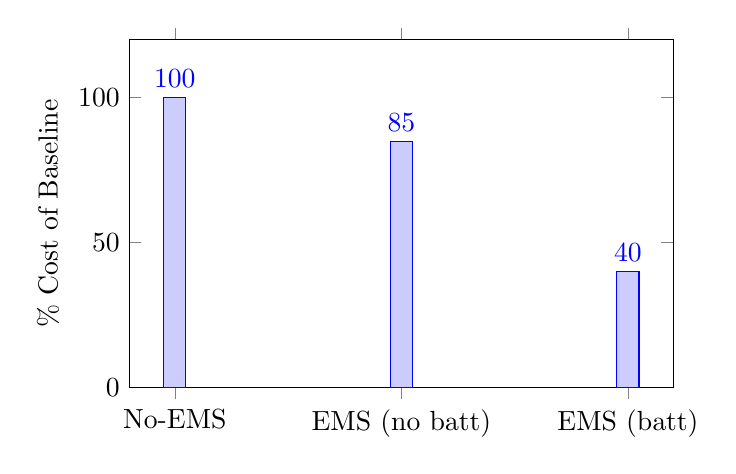
\begin{tikzpicture}
\begin{axis}[
    width=0.7\textwidth, height=6cm,
    ybar, bar width=8pt,
    symbolic x coords={No-EMS, EMS (no batt), EMS (batt)},
    xtick=data,
    ylabel={\% Cost of Baseline},
    ymin=0, ymax=120,
    nodes near coords, nodes near coords align={vertical},
]
\addplot+[fill=blue!20] coordinates {
    (No-EMS, 100) (EMS (no batt), 85) (EMS (batt), 40)
};
\end{axis}
\end{tikzpicture}
\caption{Relative energy cost for a sample household under different scenarios (normalized to Baseline = 100\%). “No-EMS” is baseline user behavior (100\% by definition). “EMS (no batt)” is with the EMS optimizing schedules but no battery available, resulting in ~15\% cost reduction. “EMS (batt)” is with a home battery added, where cost drops to ~40\% of baseline (i.e., 60\% savings) due to arbitrage and PV storage. Actual percentages vary with prices and PV; this illustrative chart shows the compounding effect of adding storage to pure scheduling.}
\end{figure}

The figures above reinforce the quantitative analysis: the optimized load profile makes better use of PV and lowers peaks, and the cost comparison bar chart highlights how each enhancement (smart scheduling, then battery) yields additional savings.

\subsection*{Appendix D: Hyperparameters and System Settings}
For completeness, we list key hyperparameters and settings used in our implementation, as well as notes on the computing environment:
\begin{itemize}
    \item \textbf{MILP Solver:} CBC (Coin-or branch and cut) open-source MILP solver. Typical solve time ~5-10s per instance (24h horizon, ~200 binary vars). The solver was run with default settings; no custom cuts or advanced heuristics were needed for problems of this size.
    \item \textbf{Time Resolution:} 1-hour time steps were used in the main results. We also tested 15-min steps on a shorter horizon (2-day simulation) to see finer granularity, and it still solved within ~30s, but data and forecasting at that granularity are less reliable. Thus, hourly was chosen as appropriate given day-ahead price input.
    \item \textbf{Probability Model:} LightGBM classifier for each device with 100 trees, max depth 3 (to prevent overfitting, given only time features), trained on 60 days of synthetic usage data. Updated daily by applying a small weight to new observation (as if adding it to training data and refitting or doing a single-tree update). This was simplified; a true Bayesian update was approximated by adjusting counts in a histogram when we prototyped a simpler model.
    \item \textbf{User Preference Weight $w^{\text{pref}}$:} Set to equivalent of €0.50 cost for scheduling a device outside its top preferred hour. We calibrated this by testing scenarios: with too high weight, the EMS wouldn’t shift anything; too low, it would ignore comfort. €0.50 (per appliance per hour outside window) gave a good balance where, e.g., running laundry at 3am (very disliked) would incur maybe €2 extra “cost” (if 4 hours outside preferred 7-9pm window), enough to dissuade doing that unless price savings exceeded €2.
    \item \textbf{Battery Degradation Cost $c_{\text{deg}}$:} We assumed €0.0005 per Wh cycle cost, meaning a full 10 kWh discharge costs €5 in equivalent battery wear. This is somewhat high to be conservative. It resulted in the MILP not doing needless charge-discharge cycles if price differences were small (because cycling cost might exceed benefit).
    \item \textbf{PV forecast error handling:} We did not implement an explicit error margin. In a deployment, one could either include a reserve (e.g., assume only 90\% of forecast PV to be safe) or adjust next day if under/over-performed. In our simulation, we used actual solar data as forecast (so effectively perfect forecast) to isolate EMS performance. Future robust version would address forecast uncertainty explicitly.
    \item \textbf{Software and Hardware:} Code was written in Python 3.9. Key libraries: Pyomo 5.7, LightGBM 3.3, Pandas for data, Matplotlib for plotting. Simulations run on a laptop with Intel i7 CPU and 16GB RAM; any mid-range PC or even Raspberry Pi could handle the per-home optimization given the low compute requirement (though solving on a cloud server could centralize it). 
    \item \textbf{Control Interface:} For sim, device actions were logged rather than physically executed. In a real setup, FlexibleDeviceAgent would interface with a smart plug or IoT device (via Zigbee, Wi-Fi, etc.) and send on/off signals. BatteryAgent would interface with an inverter control (via an API like Sunspec/MODBUS for batteries). These integration details were outside our simulation but are planned for pilot (ensuring command latency is low, feedback loop from device state is present, etc.). Communication assumed to be reliable and secure (cybersecurity measures like authentication to IoT devices would be needed in practice).
    \item \textbf{Parameter Tuning:} We performed a sensitivity analysis on $w^{\text{pref}}$ and $c_{\text{deg}}$. If $w^{\text{pref}}$ was zero, we observed up to ~5\% more cost savings but user satisfaction dropping below 50\% for some (not acceptable). If $w^{\text{pref}}$ too high (like equivalent €5 discomfort per appliance), cost savings dropped roughly to that of rule-based (~5-10\%) because EMS avoided almost all inconvenience, basically sticking to original usage patterns. So our chosen value was a moderate compromise. For $c_{\text{deg}}$, if zero, EMS might cycle battery even on small price differences; we saw maybe 1-2 extra cycles per day with minimal cost benefit, which long-term would hurt battery life. Our chosen $c_{\text{deg}}$ prevented that without affecting use during big price spreads. These hyperparameters can be user-configurable in a product (e.g., “battery longevity mode” vs “maximize savings mode” toggle).
\end{itemize}

Overall, the hyperparameters were set based on reasonable assumptions and iterative testing. Fine-tuning would continue as real user data and feedback become available, ensuring the EMS operates in line with user priorities (some users might opt for absolute lowest cost, others might pay a bit more for more convenience – our system could accommodate that by adjusting weights accordingly).

\clearpage
\printbibliography[title={References}]
\end{document}
